%!TEX root = ../template.tex
%%%%%%%%%%%%%%%%%%%%%%%%%%%%%%%%%%%%%%%%%%%%%%%%%%%%%%%%%%%%%%%%%%%%
%% chapter9.tex
%% NOVA thesis document file
%%
%% Chapter with the system validation, tests and results.
%%%%%%%%%%%%%%%%%%%%%%%%%%%%%%%%%%%%%%%%%%%%%%%%%%%%%%%%%%%%%%%%%%%%
\chapter{System Validation}
\label{cha:system_validation}

\begin{quotation}
\begin{flushright}
\itshape
«In theory there is no difference between theory and practice.\\ But in practice, there is.»\\
\textbf{- Benjamin Brewster}
\end{flushright}
\end{quotation}

The present chapter describes the system validation tests setup. Which tests are conducted and what they consist in. It follows with the exposition of the simulation test results. At the end, the results obtained are discussed.

% ==========================
% = Physical Description =
% ==========================

\section{Validation Tests Setup}
\label{sec:system_validation_tests_setup}

There were two levels of testing. The first level is testing at module level. Each component's layers were tested individually. The second level is integration testing where the whole system was tested to accomplish the goal of semi-autonomous wound filling 3D bioprinting. The test list is the following:

\begin{itemize}
    \item \textbf{First Level}
    \begin{itemize}
        \item Wound detection \& segmentation
        \item Camera spatial data processing
        \item Path planning
    \end{itemize}
    \item \textbf{Second Level}
    \begin{itemize}
        \item 3D bioprinting directly on wound
    \end{itemize}
\end{itemize}

\subsection{Wound Detection \& Segmentation}
\label{subsec:system_validation_tests_setup_wound_detection_segmentation}

Wound detection \& segmentation is all about using an algorithm that feeds on camera \gls{rgb} image data and is able indicate the location of a wound on that image.\\

\textbf{Test description}\\
The test consists in placing a wound model within the camera \gls{fov} and running an algorithm to detect and segment that wound. The wound model is a black coloured shape located on a body model section.

Five wound models, with different shapes and locations, were created and placed on a full adult human 3D model. (Fig. \ref{fig:system_validation_tests_setup_wound_detection_segmentation_wound_models}). All the wound models are non-planar surfaces. 

\begin{figure}[htbp]
	\centering
	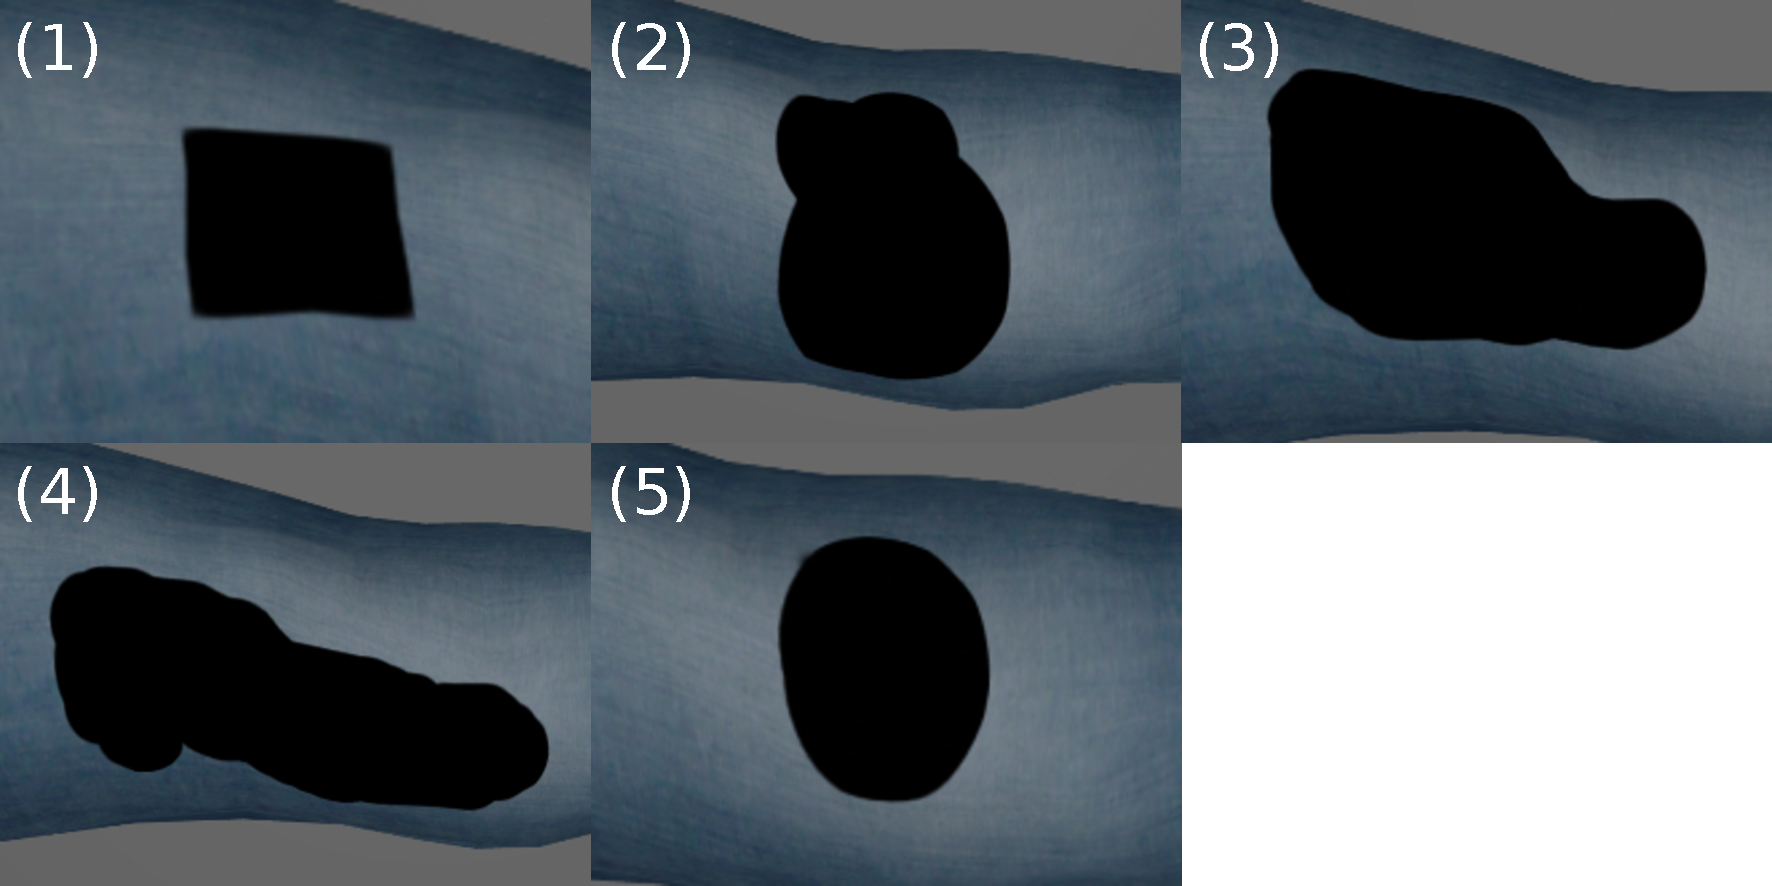
\includegraphics[width=\textwidth]{system_validation_tests_setup_wound_detection_segmentation_wound_models}
	\caption[Wound models used to test wound detection and segmentation.]{Wound models used to test wound detection and segmentation.}
	\label{fig:system_validation_tests_setup_wound_detection_segmentation_wound_models}
\end{figure}

% subsection system_validation_tests_setup_wound_detection_segmentation

\subsection{Camera Spatial Data Processing}
\label{subsec:system_validation_tests_setup_camera_spatial_data_processing}

The wound position is needed to control the positioning system. Other geometrical information may be important like area and perimeter. Because non-planar surfaces are considered, a mesh of the wound model is also created. Each data type has its own test.

\subsubsection*{Wound Position}
\label{subsubsec:system_validation_tests_setup_camera_spatial_data_processing_position}

This test uses a square wound model with a predefined position is space and dimensions. After detection and segmentation of this wound, the position is calculated using the algorithm described in \textbf{Spatial Data Processing} layer on subsection \ref{subsubsec:system_architectural_camera_layers_spatial_data}. The data obtained is compared with the predefined values.

The wound models on this test are placed on the robot base plane. They are all quadrilateral to simplify the area and perimeter calculations. The first is a square of $0.1\times0.1$ \si{\meter} centered at position (0.65, 0, 0.1) \si{\meter}, referenced to robot base frame. The second and third are rectangles, $0.1\times0.2$ \si{\meter} centered at position (0.7, -0.1, 0.1) \si{\meter}, and $0.15\times0.05$ \si{\meter} centered at position (0.6, 0.1, 0.08) \si{\meter}.

\subsubsection*{Wound Area \& Perimeter}
\label{subsubsec:system_validation_tests_setup_camera_spatial_data_processing_area_perimeter}

For the area test everything was the same as the position test, except the calculation. The wound perimeter test is similar to wound position and area tests. The only change is the calculation of the wound perimeter.
 
% subsubsection system_validation_tests_setup_camera_spatial_data_processing_area_perimeter

\subsubsection*{Wound Mesh}
\label{subsubsec:system_validation_tests_setup_camera_spatial_data_processing_mesh}

To test wound mesh generation, the wound models used were the same as the ones used for wound detection and segmentation tests.

The test uses the point data from wound segmentation and applies an algorithm to generate a wound mesh. The validation is done through visual comparison of the mesh shape and wound model shape.
 
% subsubsection system_validation_tests_setup_camera_spatial_data_processing_mesh

% subsection system_validation_tests_setup_camera_spatial_data_processing

\subsection{Path Planning}
\label{subsec:system_validation_tests_setup_path_planning}

The path planning is essential to define a robot movement capable of direct wound filling 3D bioprinting. The 3 different paths provided must be validated for proper execution.\\

\textbf{Test description}\\
The wound models are the same as the ones for wound detection and segmentation tests. For each wound model, the three path planning algorithms are applied.

% subsection system_validation_tests_setup_path_planning

\subsection{3D Bioprinting Directly on Wound}
\label{subsec:system_validation_tests_setup_bioprinting_directly_wound}

The final test comprises a combination of all the previous functionalities to reach the end goal of bioprinting directly on a wound.\\

\textbf{Test description}\\
For these tests, the five wound models will be used. The test has the following steps:

\begin{enumerate}
    \item Position wound into camera FOV;
    \item Run wound detection \& segmentation;
    \item Process wound spatial data;
    \item Generate wound filling path and trajectory;
    \item Execute trajectory.
\end{enumerate}

% subsection system_validation_tests_setup_bioprinting_directly_wound

% section system_validation_tests_setup

% ==========================
% = Simulation Results =
% ==========================

\section{Simulated System Results}
\label{sec:system_validation_simulation_results}

On this section, the results for simulated environment tests are presented. The tests were conducted on Gazebo robot simulator. Gazebo uses a physical simulation engine, advanced 3D graphics, and supports various sensors and robot models. For more information about Gazebo and system setup on Gazebo refer to appendix \ref{app:gazebo_setup}.

The environment consists on a virtual patient room. In it, a patient is lying on bed and the robotic arm lies by the bed side. The room setup tries to replicate a normal patient room with some common hospital apparel (Fig. \ref{fig:system_validation_simulation_gazebo_environment}).

\begin{figure}[htbp]
	\centering
	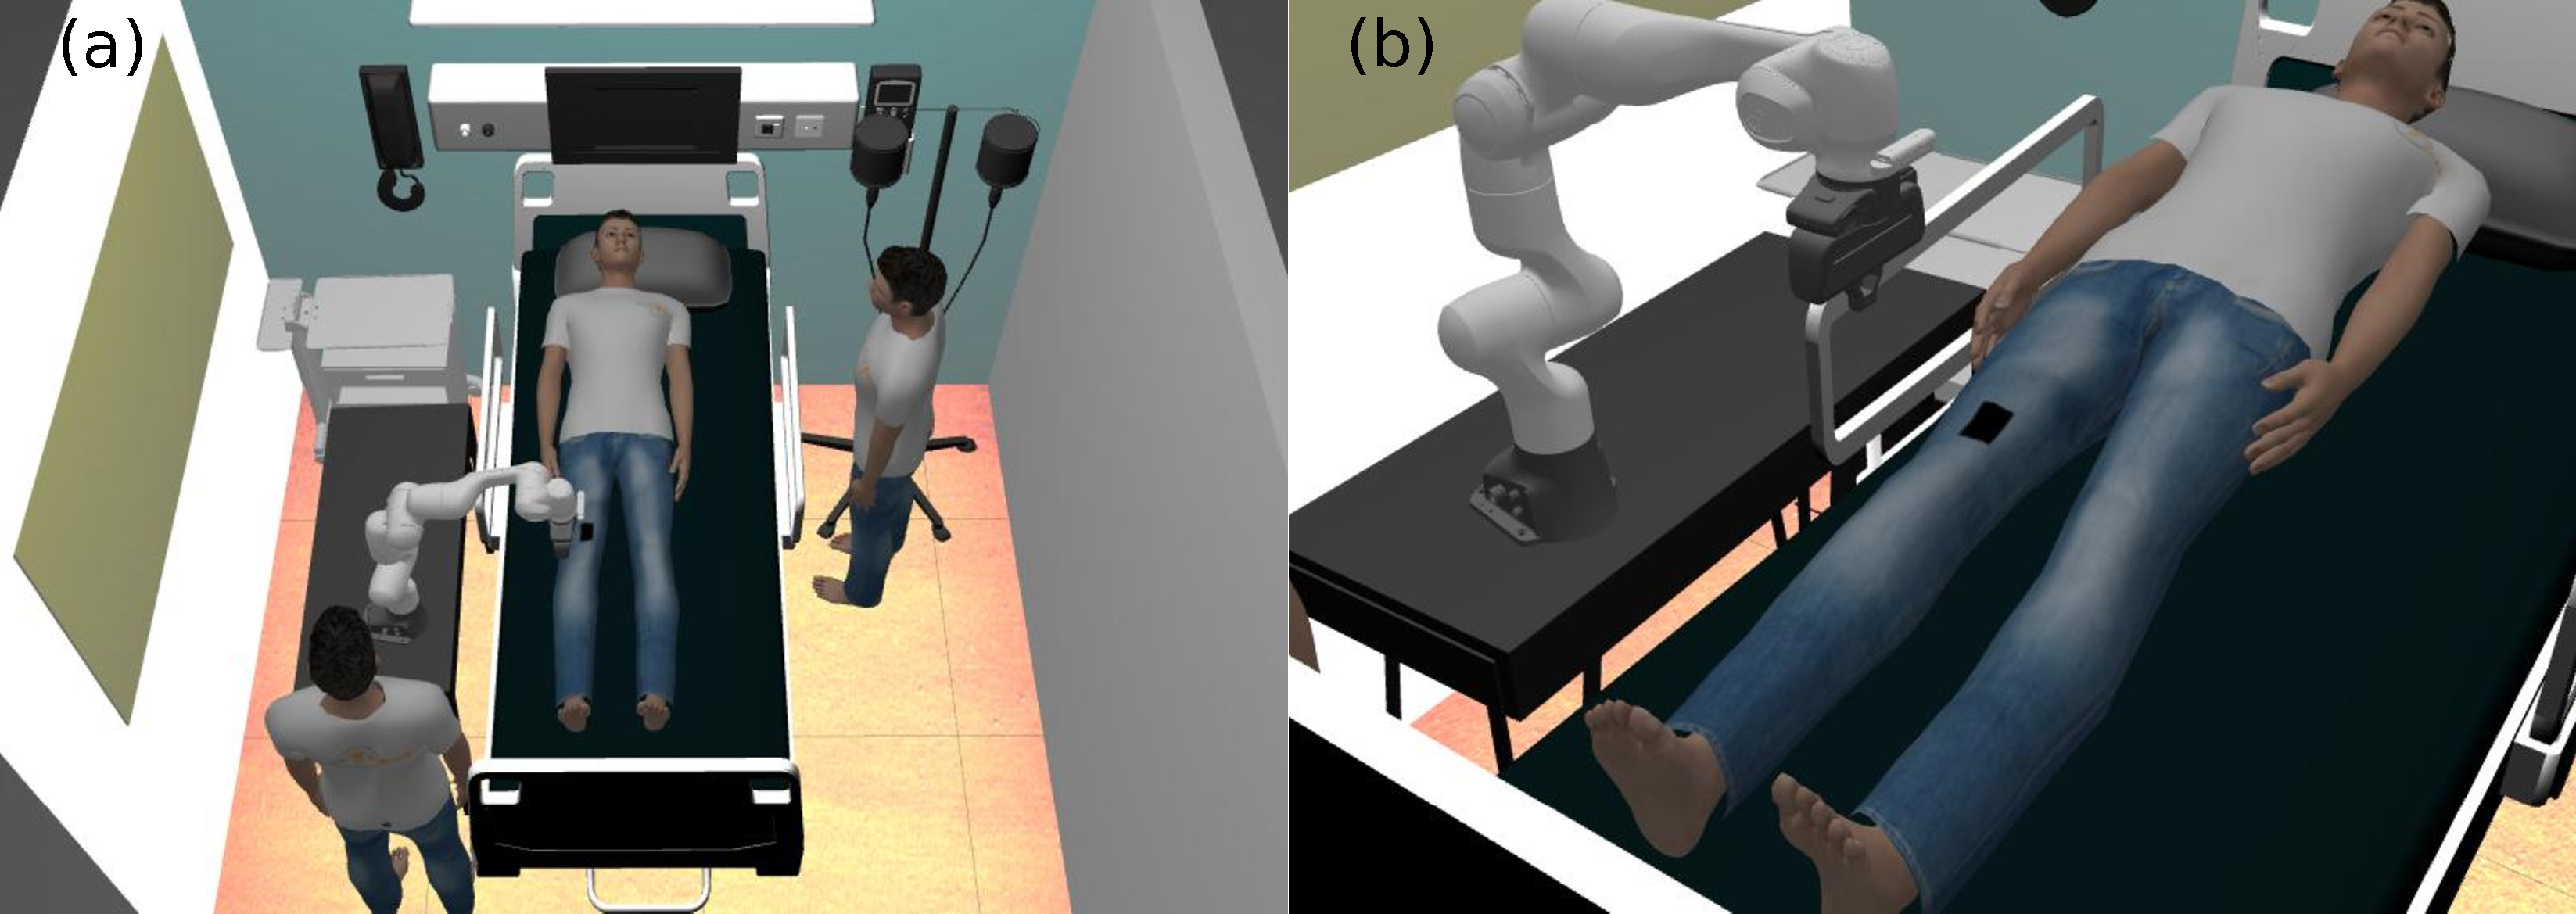
\includegraphics[width=\textwidth]{system_validation_simulation_gazebo_environment}
	\caption[Simulated environment on Gazebo Simulator.]{Simulated environment on Gazebo Simulator. (a) Top-view of the patient room. Gives an overall view of the room's apparel organisation. The standing human models represent clinicians. (b) Close-up on robot and patient. The wound model is better visible and its spacial relation with the patient and robot.}
	\label{fig:system_validation_simulation_gazebo_environment}
\end{figure}

\subsection{Wound Detection \& Segmentation}
\label{subsec:simulated_system_results_wound_detection_segmentation}

After running the camera detection and segmentation algorithm on the five wound models supplied, the following results were obtained (Fig. \ref{fig:system_validation_simulation_results_wound_detection_segmentation}).\\

\begin{figure}[htbp]
	\centering
	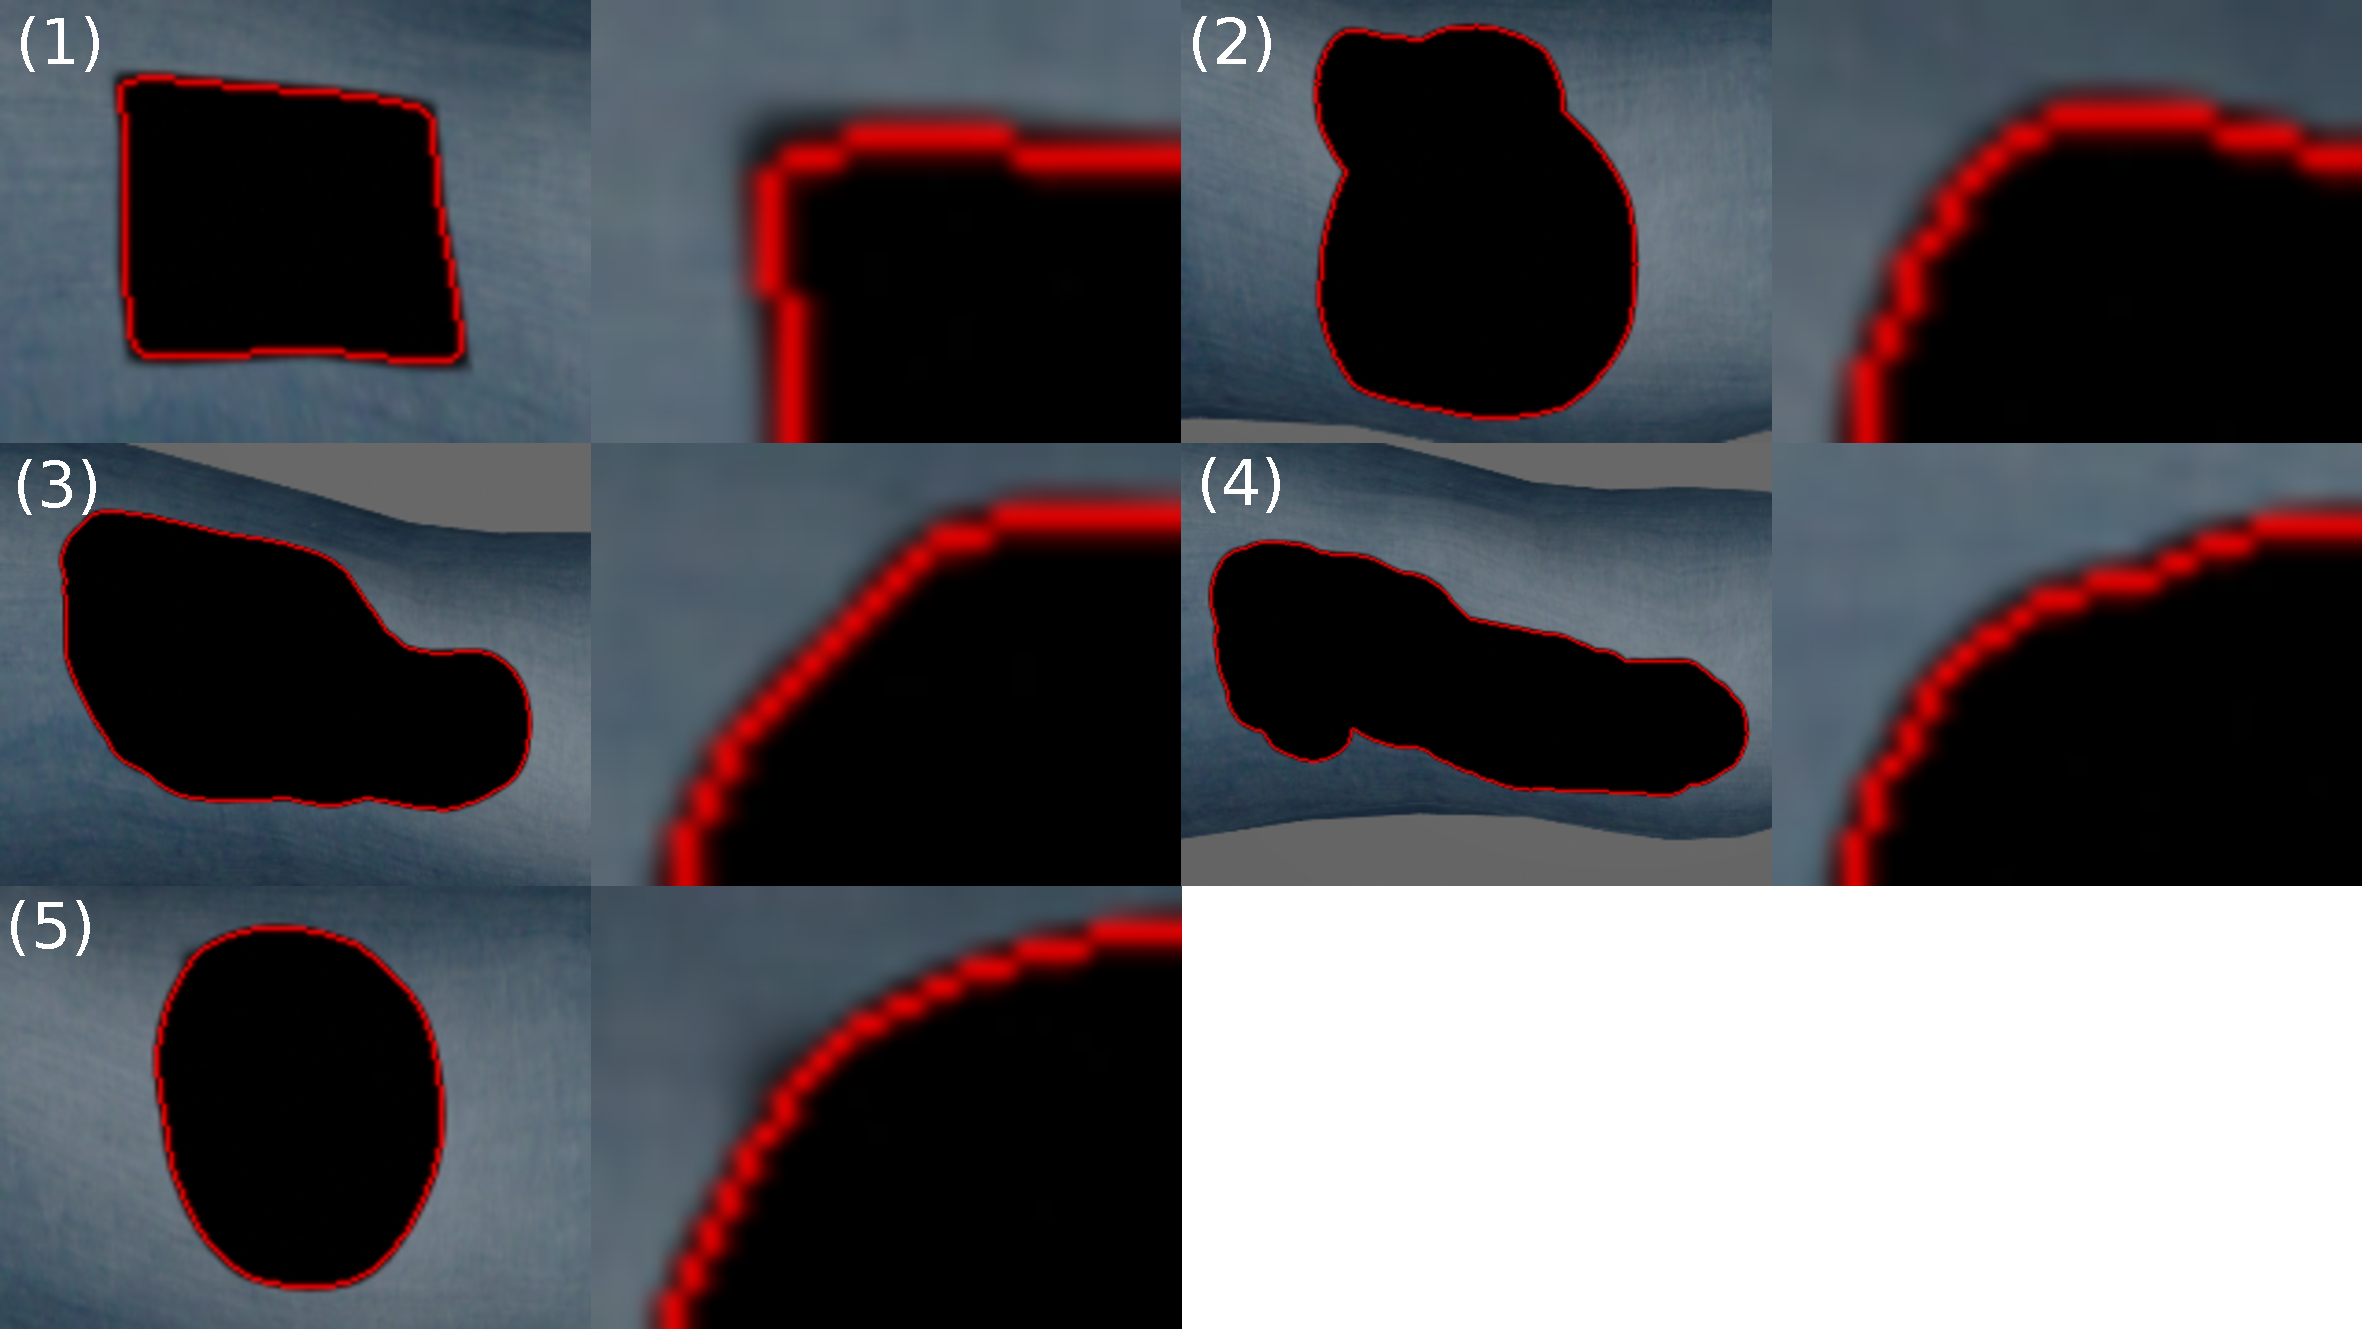
\includegraphics[width=\textwidth]{system_validation_simulation_results_wound_detection_segmentation}
	\caption[Simulated system wound detection \& segmentation results.]{Simulated system wound detection \& segmentation results. The red lines are the detected wound contours. Each model has a full image (left) and a detailed crop (right) to see the wound-contour edge relation. It is visible that for every wound model the contour encloses the whole wound.}
	\label{fig:system_validation_simulation_results_wound_detection_segmentation}
\end{figure}

On all models, the algorithm was able to correctly detect the wound model and segment it. The segmentation contour encloses the whole wound area as desired. The zoomed areas for each wound show that the contour goes all the way to the edge of the wound model.

% subsection simulated_system_results_wound_detection_segmentation

\subsection{Camera Spatial Data Processing}
\label{subsec:simulated_system_results_camera_spatial_data_processing}

Camera spatial data processing encompasses various tests. The results will be presented for each test separately.

\subsubsection*{Wound Position}
\label{subsubsec:simulated_system_results_camera_spatial_data_processing_position}

The wound position data for the three quadrilateral wound models is presented on table \ref{tab:wound_position_results}. Figure \ref{fig:simulation_test_results_camera_spatial_data_wound_position_test_results} shows the relation between the camera point cloud and the wound detected point cloud.

As the figure shows, there was a mismatch between the point cloud generated by the segmentation algorithm and the real point cloud. This means the robot will not be able to execute the right wound filling trajectory.

\begin{table}[htbp]
    \centering
    \caption[Wound position data.]{Wound position data. Tx and Ty are the true x and true y. Each line represents a quadrilateral corner point.}
    \begin{tabular}{c|c|c|c|c|c}
        \toprule
         \textbf{Tx (m)} & \textbf{Ty (m)} & \textbf{x (m)} & \textbf{y (m)} & \textbf{|Tx-x| (m)} & \textbf{|Ty-y| (m)} \\
         \midrule
         \multicolumn{6}{c}{Wound 1} \\
         \midrule
         0.7000 & 0.0500 & 0.6827 & 0.0321 & 0.0173 & 0.0179 \\
         0.6000	& 0.0500 & 0.6109 &	0.0316 & 0.0109	& 0.0184 \\
         0.6000	& -0.0500 &	0.6104 & -0.0402 & 0.0104 &	0.0098 \\
         0.7000	& -0.0500 &	0.6831 & -0.0406 & 0.0169 &	0.0094 \\
         \midrule
         \multicolumn{6}{c}{Wound 2} \\
         \midrule
         0.7500	& 0.0000 & 0.7280 &	-0.0030 & 0.0220 & 0.0030 \\
         0.6500	& 0.0000 & 0.6450 &	-0.0030 & 0.0050 & 0.0030 \\
         0.6500	& -0.2000 &	0.6450 & -0.1653 & 0.0050 & 0.0347 \\
         0.7500	& -0.2000 &	0.7280 & -0.1653 & 0.0220 & 0.0347 \\
         \midrule
         \multicolumn{6}{c}{Wound 3} \\
         \midrule
         0.6750	& 0.1250 & 0.6686 &	0.0934 & 0.0064 & 0.0316 \\
         0.5250	& 0.1250 & 0.5490 & 0.0943 & 0.0240 & 0.0307 \\
         0.5250	& 0.0750 & 0.5490 & 0.0476 & 0.0240	& 0.0274 \\
         0.6750	& 0.0750 & 0.6686 & 0.0476 & 0.0064	& 0.0274 \\
         \bottomrule
    \end{tabular}
    \label{tab:wound_position_results}
\end{table}

\begin{figure}[htbp]
	\centering
	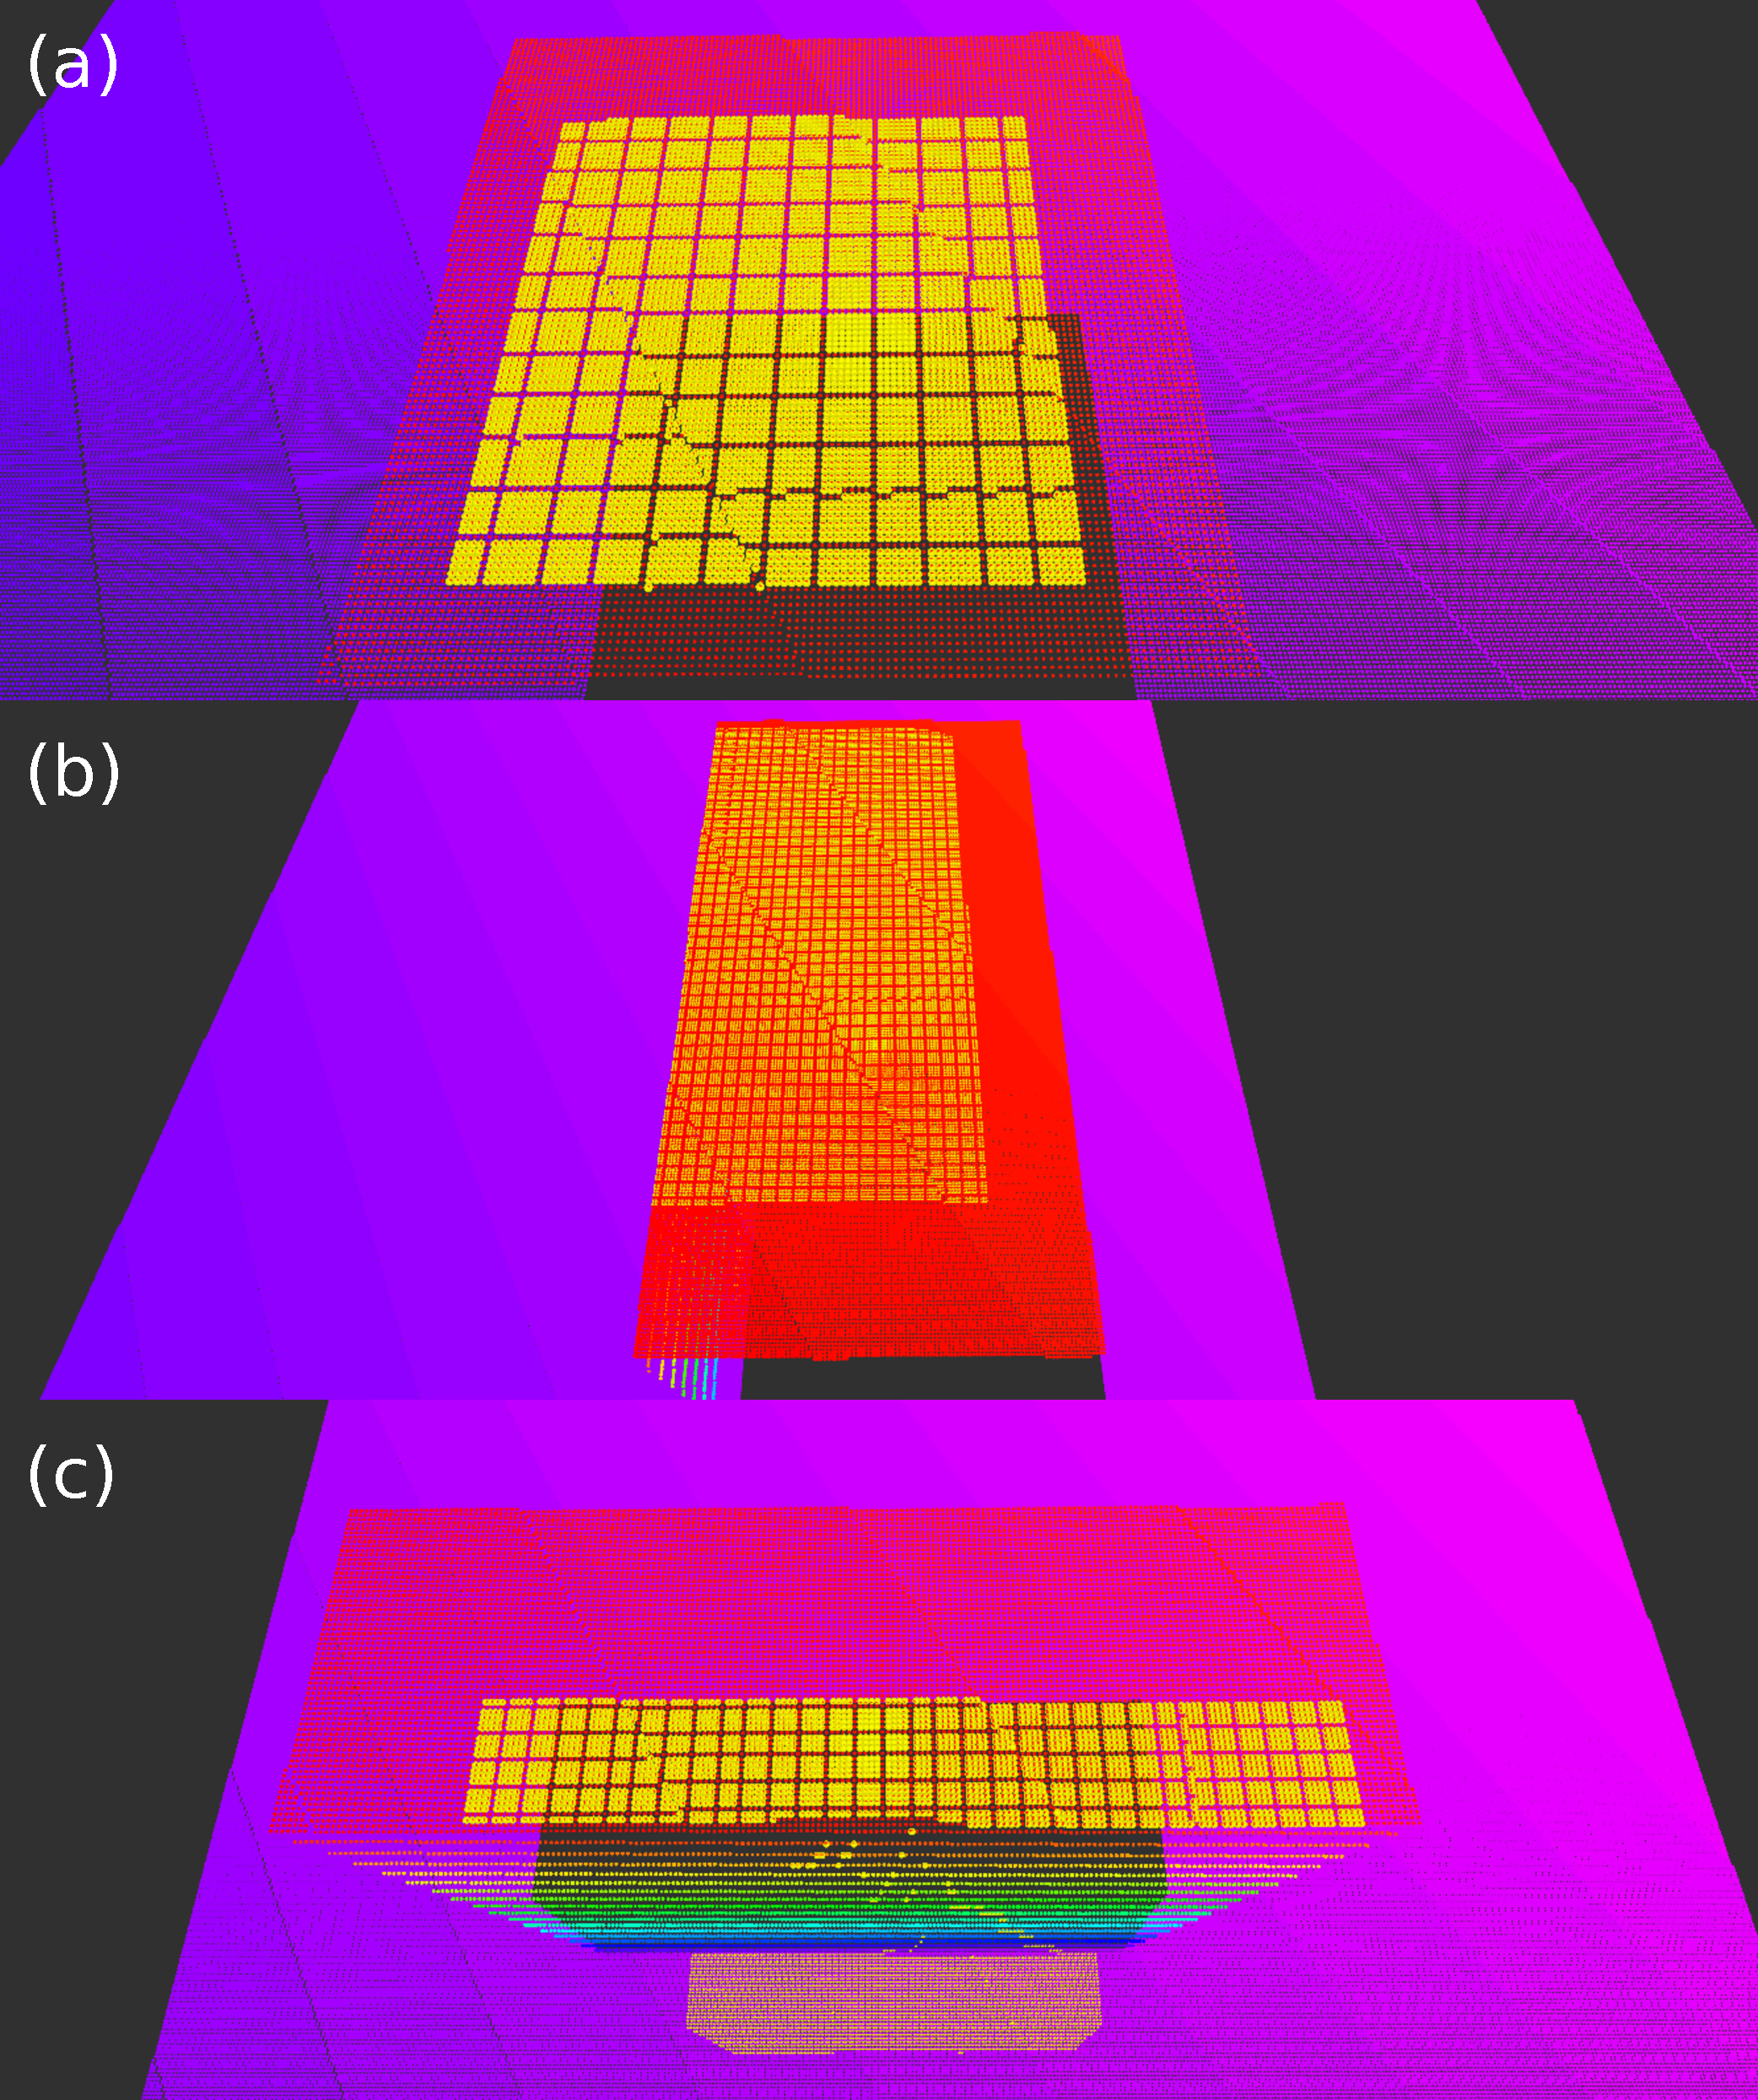
\includegraphics[width=0.7\textwidth]{wound_position_test_results}
	\caption[Wound position test results.]{Wound position test results. Each image shows the relation between the camera point cloud (red area) and the wound point cloud detected by the segmentation algoritm (yellow are). (a) Wound model 1, $0.1\times0.1$ \si{\meter}. (b) Wound model 2, $0.1\times0.2$ \si{\meter}. (c) Wound model 3, $0.15\times0.05$ \si{\meter}.}
	\label{fig:simulation_test_results_camera_spatial_data_wound_position_test_results}
\end{figure}

% subsubsection simulated_system_results_camera_spatial_data_processing_position

\subsubsection*{Wound Area \& Perimeter}
\label{subsubsec:simulated_system_results_camera_spatial_data_processing_area_perimeter}

The area and perimeter data, also associated with the three quadrilateral wound models, is presented on tables \ref{tab:wound_area_results} and \ref{tab:wound_perimeter_results}.

\begin{table}[htbp]
    \centering
    \caption[Wound area data.]{Wound area data. The T prefix means true. The p prefix means values related with the position points obtained on the previous test. A is the area calculated by the area algorithm.}
    \begin{adjustbox}{width=1.2\textwidth,center=\textwidth}
    \begin{tabular}{c|c|c|c|c|c|c|c|c|c}
         \toprule
         \textbf{Wound} & \textbf{Tdx (m)} & \textbf{Tdy (m)} & \textbf{TA (\si{\meter\squared})} & \textbf{pdx (m)} & \textbf{pdy (m)} & \textbf{pA (\si{\meter\squared})} & \textbf{A (\si{\meter\squared})} & \textbf{|TA-A| (\si{\meter\squared})} & \textbf{|pA-A| (\si{\meter\squared})} \\
         1 & 0.1000 & 0.1000 & 0.0100 & 0.0727 & 0.0727 & 0.0053 & 0.0052 & 0.0048 & 0.0001 \\
         2 & 0.1000 & 0.2000 & 0.0200 & 0.0830 & 0.1623 & 0.0135 & 0.0133 & 0.0067 & 0.0002 \\
         3 & 0.1500 & 0.0500 & 0.0075 & 0.1196 & 0.0459 & 0.0055 & 0.0054 & 0.0021 & 0.0001 \\
         \bottomrule
    \end{tabular}
    \end{adjustbox}
    \label{tab:wound_area_results}
\end{table}

\begin{table}[htbp]
    \centering
    \caption[Wound perimeter data.]{Wound perimeter data. The T prefix means true. The p prefix means values related with the position points obtained on the previous test. P is the perimeter calculated by the perimeter algorithm.}
    \begin{adjustbox}{width=1.2\textwidth,center=\textwidth}
    \begin{tabular}{c|c|c|c|c|c|c|c|c|c}
         \toprule
         \textbf{Wound} & \textbf{Tdx (m)} & \textbf{Tdy (m)} & \textbf{TP (m)} & \textbf{pdx (m)} & \textbf{pdy (m)} & \textbf{pP (m)} & \textbf{P (m)} & \textbf{|TP-P| (m)} & \textbf{|pP-P| (m)} \\
         1 & 0.1000 & 0.1000 & 0.4000 & 0.0727 & 0.0727 & 0.2908 & 0.2173 & 0.1827 & 0.0735 \\
         2 & 0.1000 & 0.2000 & 0.6000 & 0.0830 & 0.1623 & 0.4906 & 0.3662 & 0.2338 & 0.1244 \\
         3 & 0.1500 & 0.0500 & 0.4000 & 0.1196 & 0.0459 & 0.3309 & 0.2426 & 0.1574 & 0.0883 \\
         \bottomrule
    \end{tabular}
    \end{adjustbox}
    \label{tab:wound_perimeter_results}
\end{table}

% subsubsection simulated_system_results_camera_spatial_data_processing_area_perimeter

\subsubsection*{Wound Mesh}
\label{subsubsec:simulated_system_results_camera_spatial_data_processing_mesh}

For the wound mesh tests, each wound model will have a point cloud and a mesh associated. The mesh is obtained from the point cloud. The point clouds are visualised on RViz. The results are presented on Figure \ref{fig:simulation_test_results_camera_spatial_data_wound_pcloud_mesh_resume}. It was not possible to create a mesh out of the wound point clouds obtained.

\begin{figure}[htbp]
	\centering
	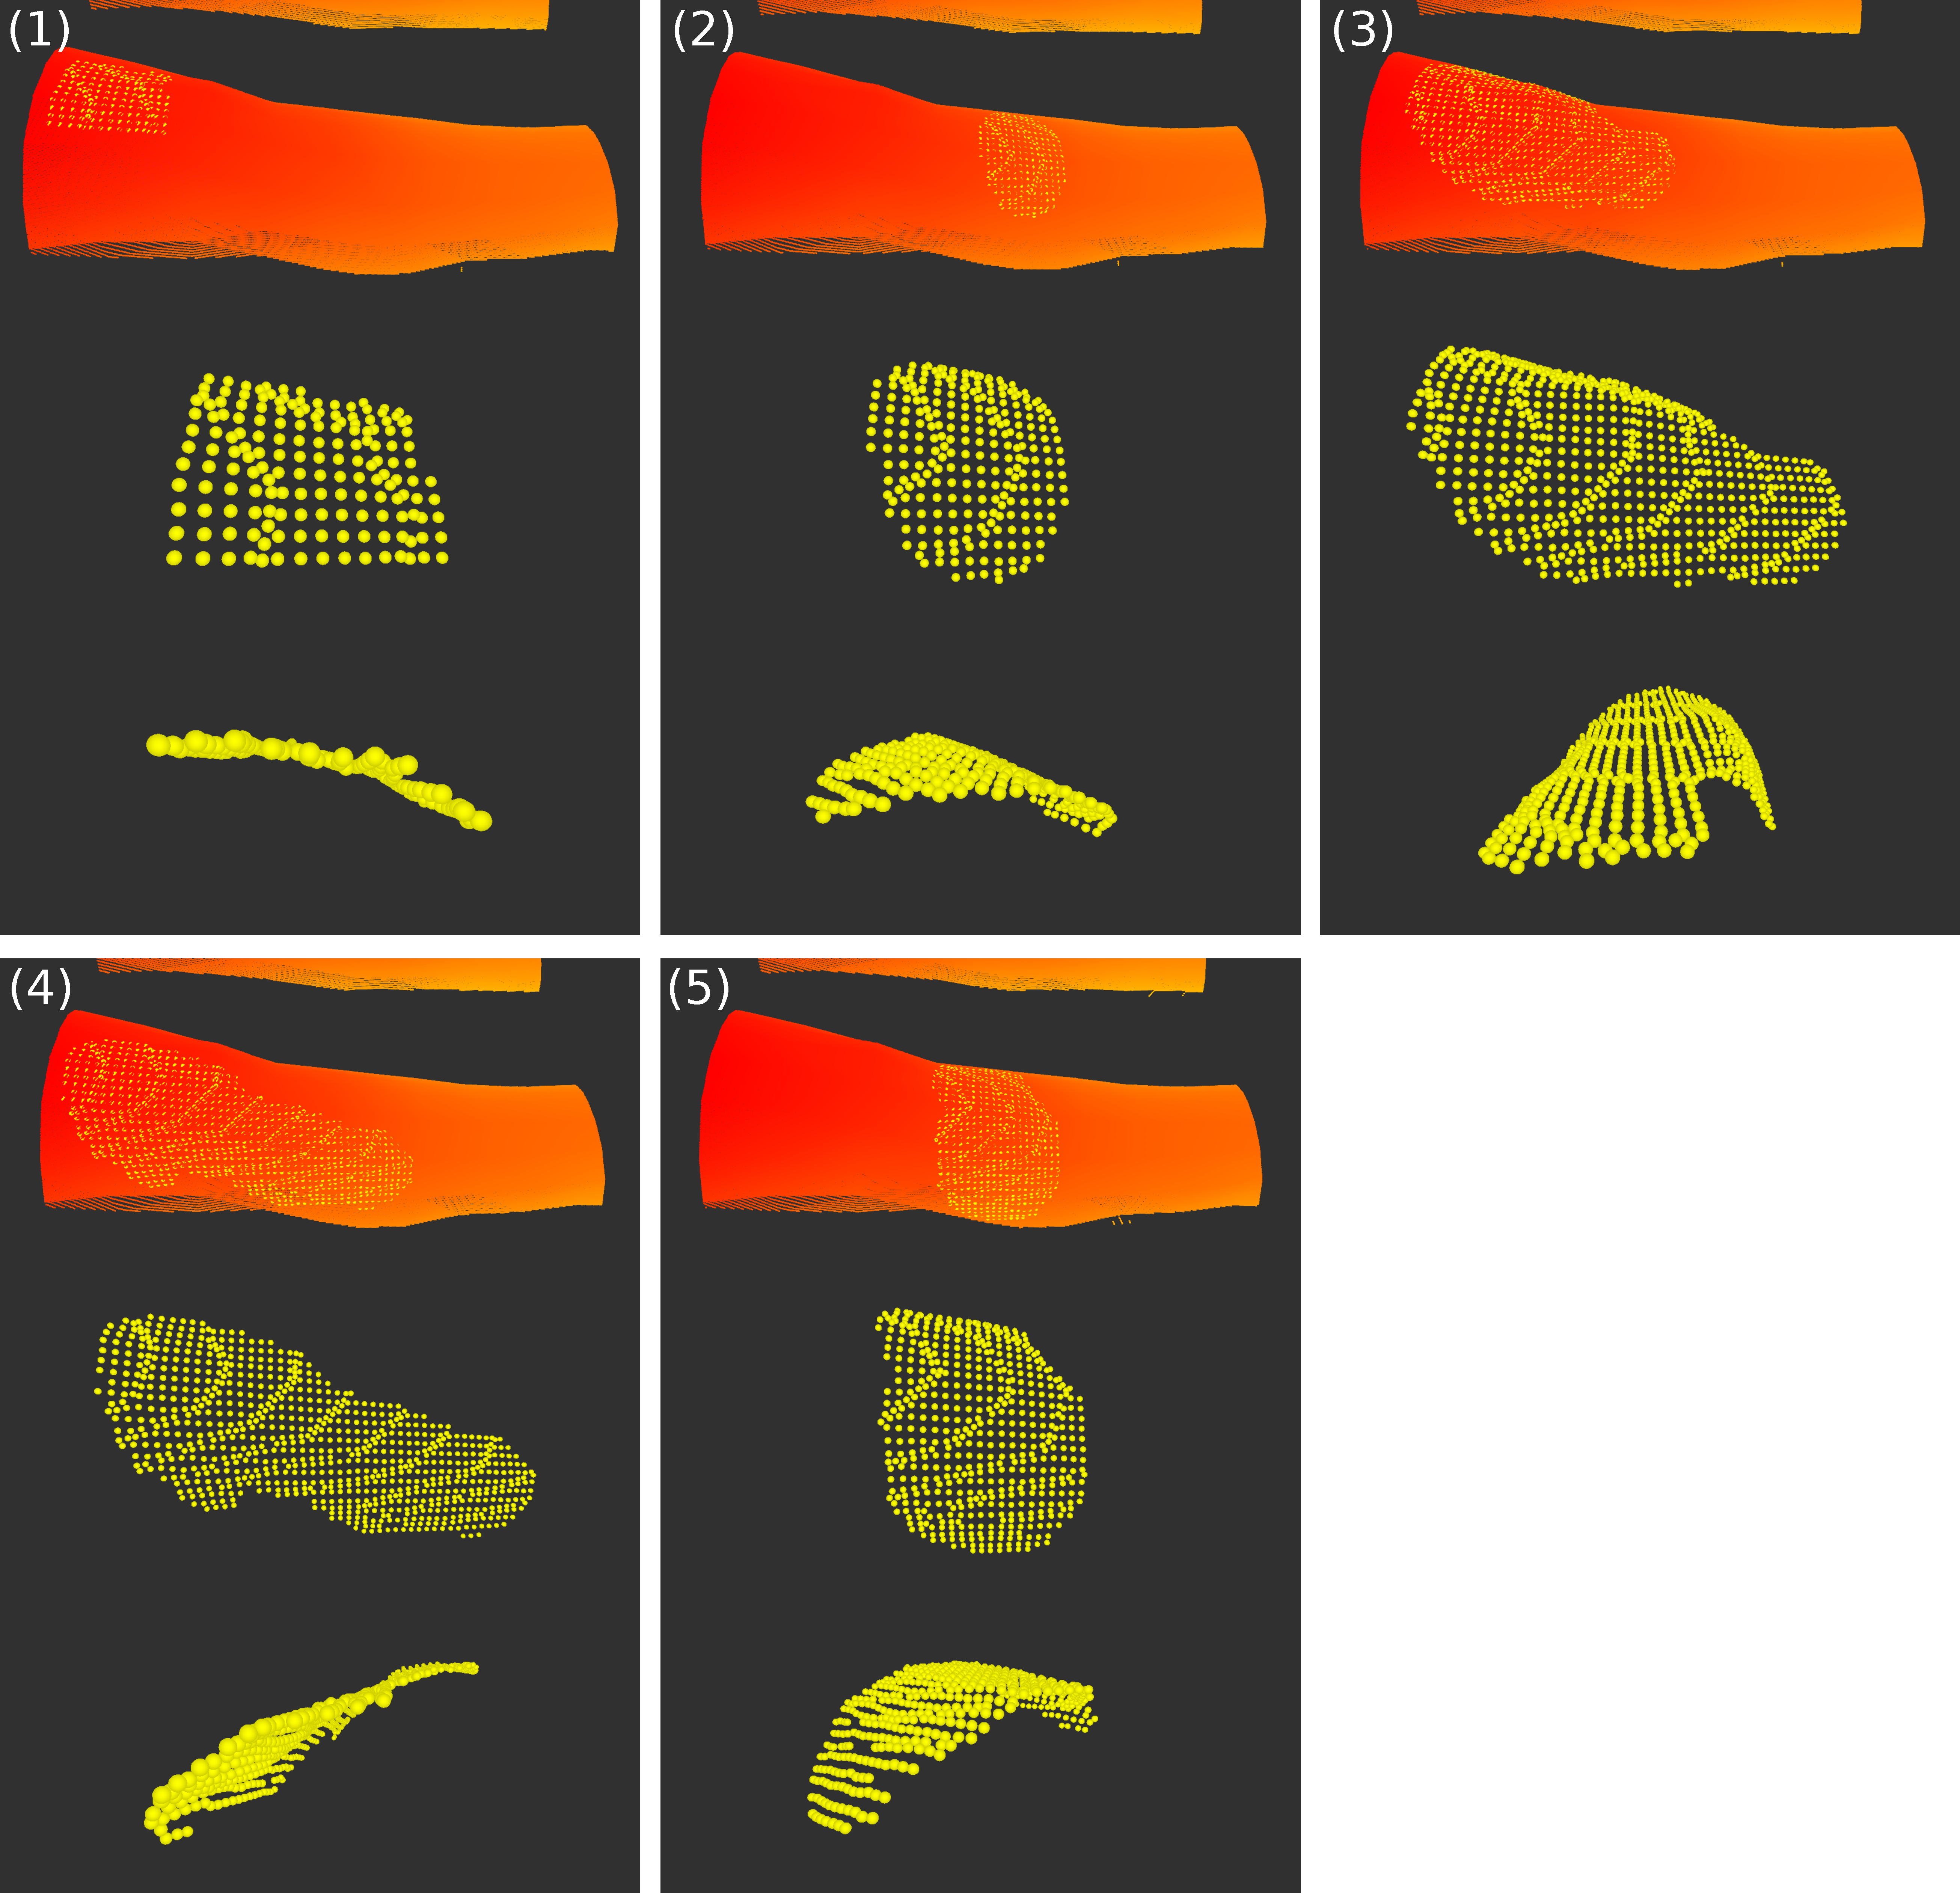
\includegraphics[width=.72\textwidth]{simulation_test_results_appendix_camera_spatial_data_pcloud}
	\caption[Wound model's point cloud.]{Wound model's point cloud. Each wound model has three representations of the associated point cloud. (top) Wound point cloud in yellow superimposed on the patient model's leg point cloud. (middle) Centred zoom on the wound point cloud. The perspective is the same as top. (bottom) Different perspective of the point cloud to evidence its non-planar nature. }
	\label{fig:simulation_test_results_camera_spatial_data_wound_pcloud_mesh_resume}
\end{figure}

% subsubsection simulated_system_results_camera_spatial_data_processing_mesh

% subsection simulated_system_results_camera_spatial_data_processing

\subsection{Path Planning}
\label{subsec:simulated_system_results_path_planning}

With the wound contour available, the path planning algorithms can be applied. Three different algorithms with the same configuration were applied to each wound model. The results are presented on Figure \ref{fig:simulation_test_results_toolpath_resume}.\\

\begin{figure}[htbp]
	\centering
	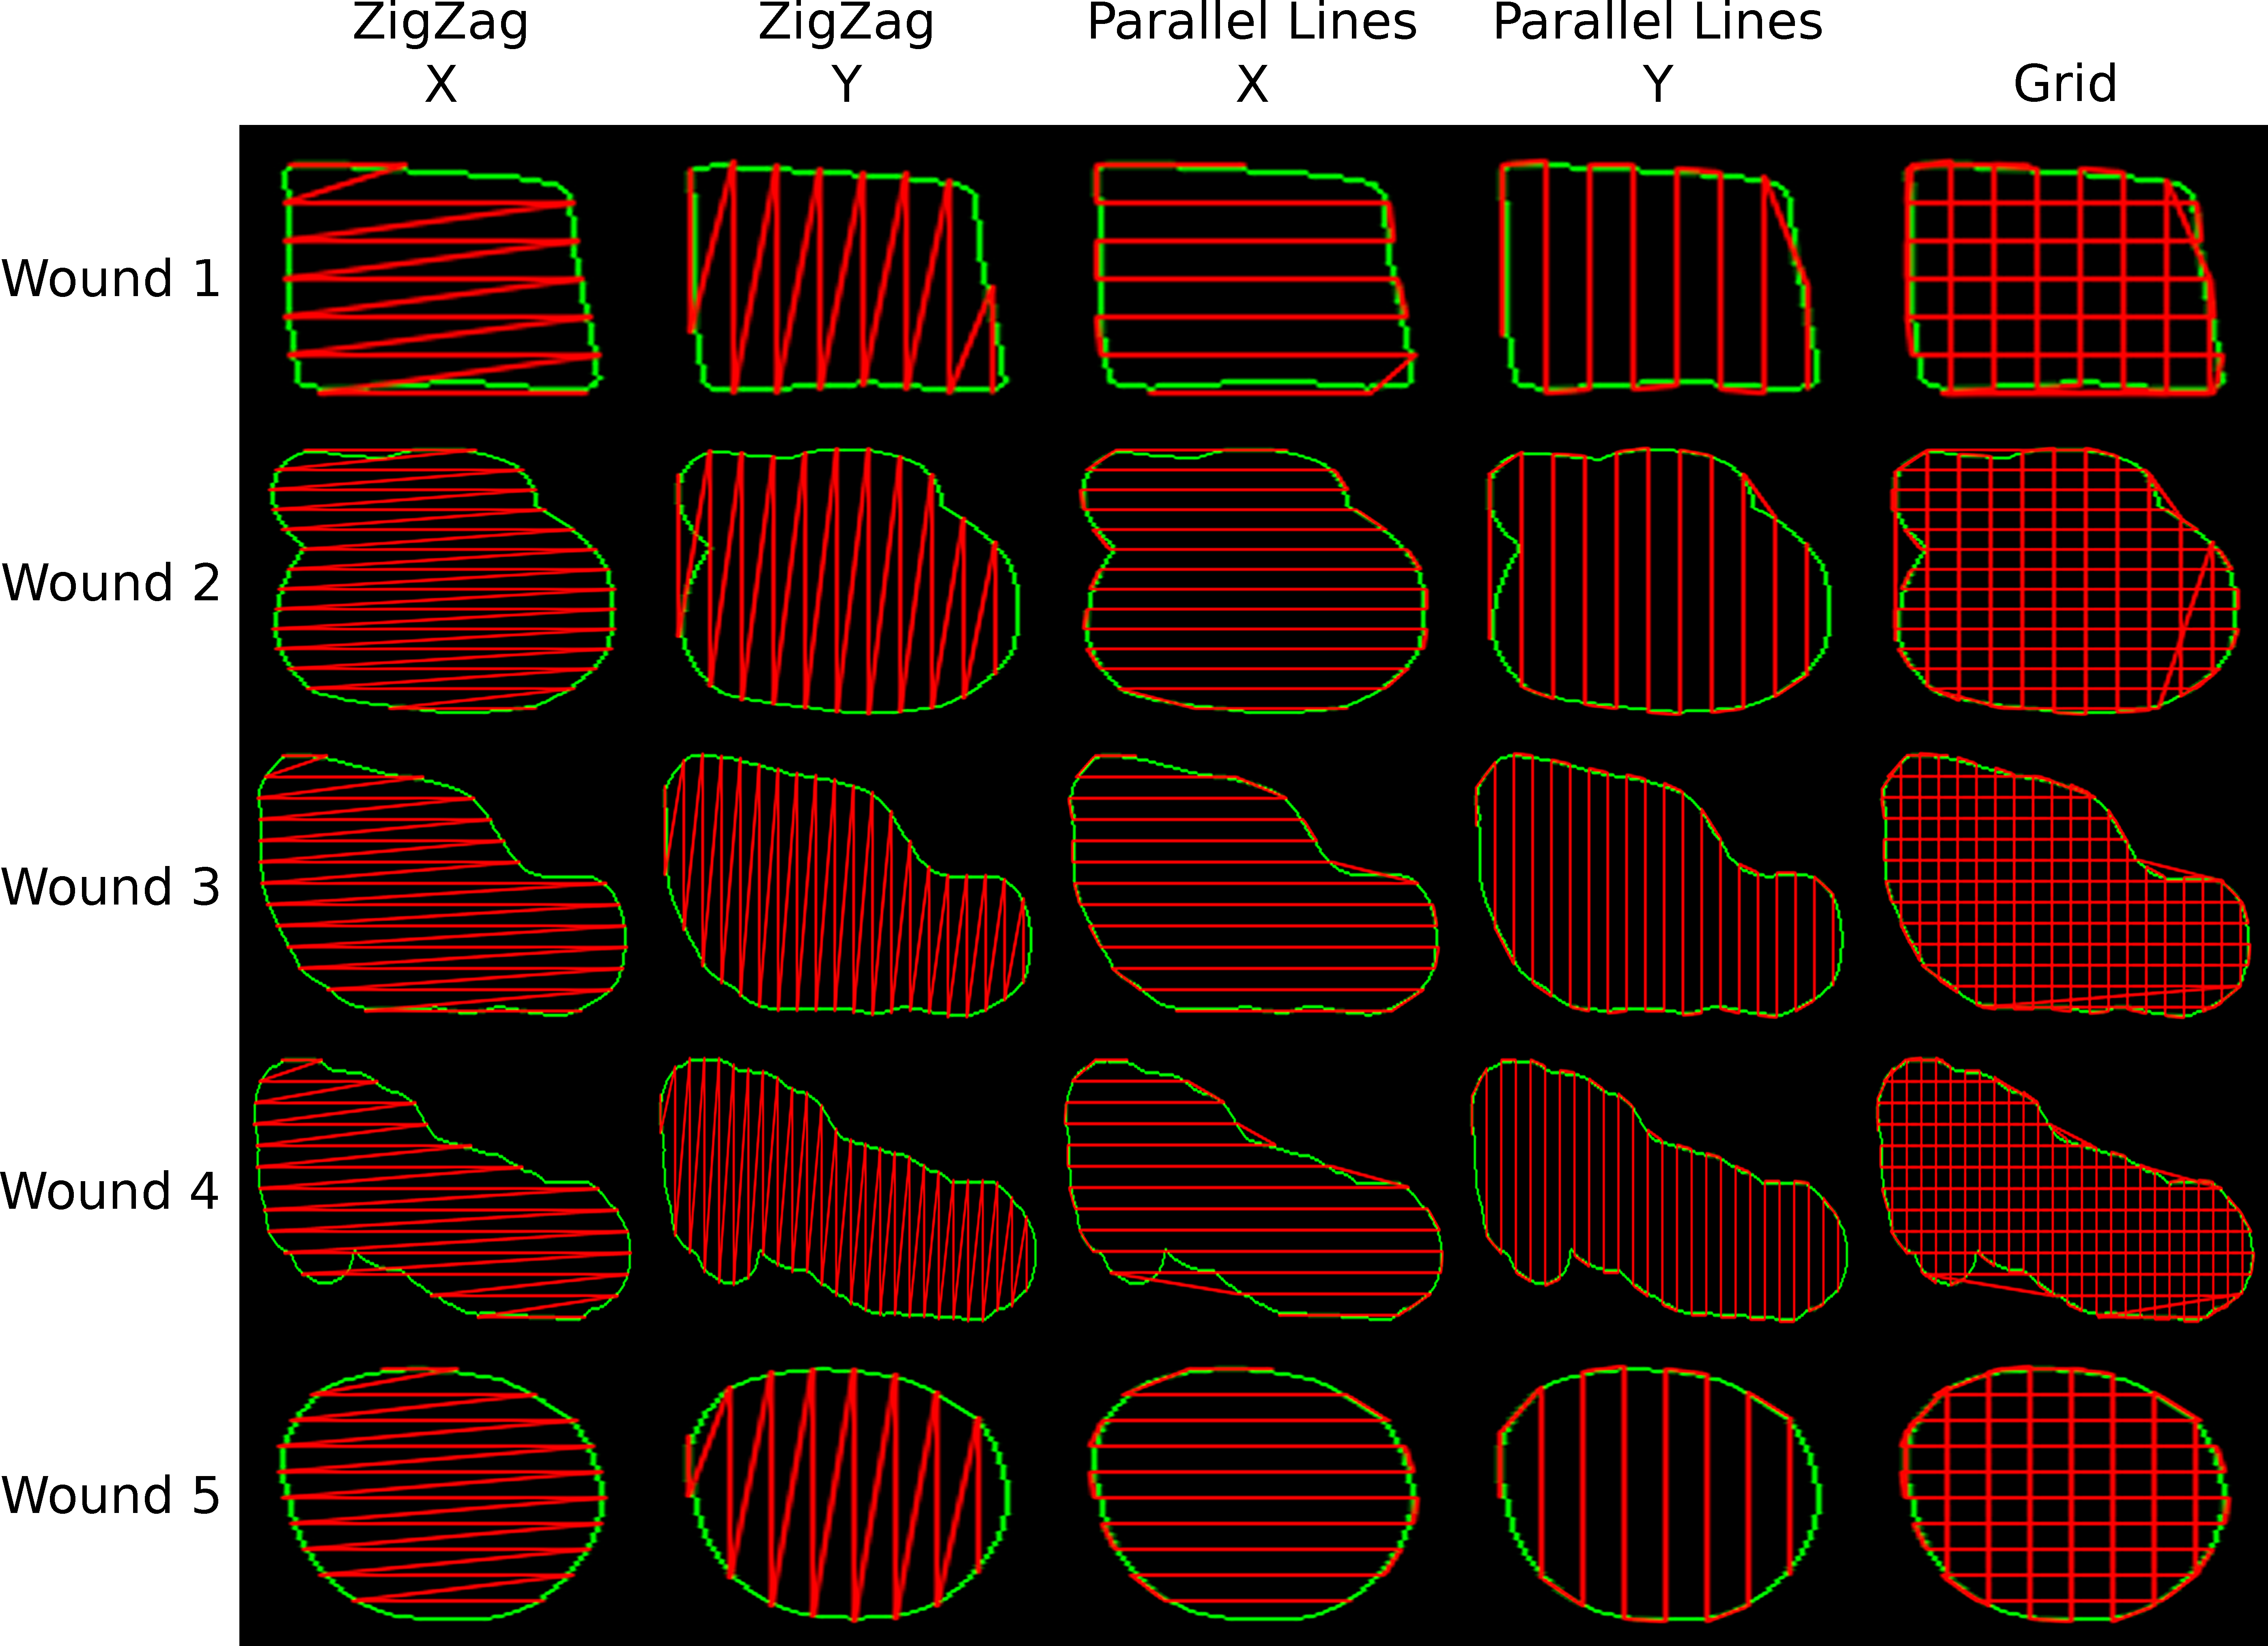
\includegraphics[width=\textwidth]{simulation_test_results_toolpath_resume}
	\caption[Simulation results for path planning.]{Simulation results for path planning. Each line represents a different wound model. From left to right, the algorithm changes. All results have a distance between lines, $L = 5$, in pixels.}
	\label{fig:simulation_test_results_toolpath_resume}
\end{figure}

All the results show that the planned paths are contained inside the wound area. They are also able to fill the wound completely. By controlling the distance $L$, various filling grades can be accomplished. The examples presented show a fixed value of $L = 5$.

However, it is important to mention that in some cases the planned path goes beyond the wound segmented area. This happens in zones where the shape is concave, but it also depends on the orientation of the algorithm and distance $L$. For example, wound 4's ZigZag X path goes outside the segmented area, while the ZigZag Y does not.

The full results with various path configurations are available on appendix \ref{app:simulation_test_results}.

% subsection simulated_system_results_path_planning

\subsection{3D Bioprinting Directly on Wound}
\label{subsec:simulated_system_results_bioprinting_directly_wound}

For the complete procedure, only the results for wound model 1 will be presented here. The complete results are available on appendix \ref{app:simulation_test_results}.

First, the cartesian impedance controller parameters used are listed on table \ref{tab:cartesian_impedance_gains}. These parameters control the end-effector position and orientation, and correspond to the diagonal values of the stiffness ($\boldsymbol{K}$), damping ($\boldsymbol{D}$) and integral ($\boldsymbol{I}$) matrices.

\begin{table}[htbp]
    \centering
    \caption[Cartesian impedance gains.]{Cartesian impedance gains.}
    \begin{tabular}{c|c|c|c}
         \toprule
         \textbf{DoF} & \textbf{K} & \textbf{D} & \textbf{I}  \\
         \midrule
         \textbf{px} & 5000 & 120 & 0.01 \\ 
         \textbf{py} & 5000 & 120 & 0.01 \\ 
         \textbf{pz} & 5000 & 120 & 0.01 \\ 
         \textbf{ox} & 200 & 10 & 0.001 \\ 
         \textbf{oy} & 200 & 10 & 0.001 \\ 
         \textbf{oz} & 200 & 10 & 0.001 \\ 
         \bottomrule
    \end{tabular}
    \label{tab:cartesian_impedance_gains}
\end{table}

Using the parameters from table \ref{tab:cartesian_impedance_gains} a 20 second trajectory was executed for each path, using $L = 5$. The visual trajectory results are shown on Figure \ref{fig:simulation_test_results_toolpath_wound_1}. Table \ref{tab:cartesian_impedance_tracking_rmse} presents the \gls{rms} error for the trajectory tracking.

\begin{figure}[htbp]
	\centering
	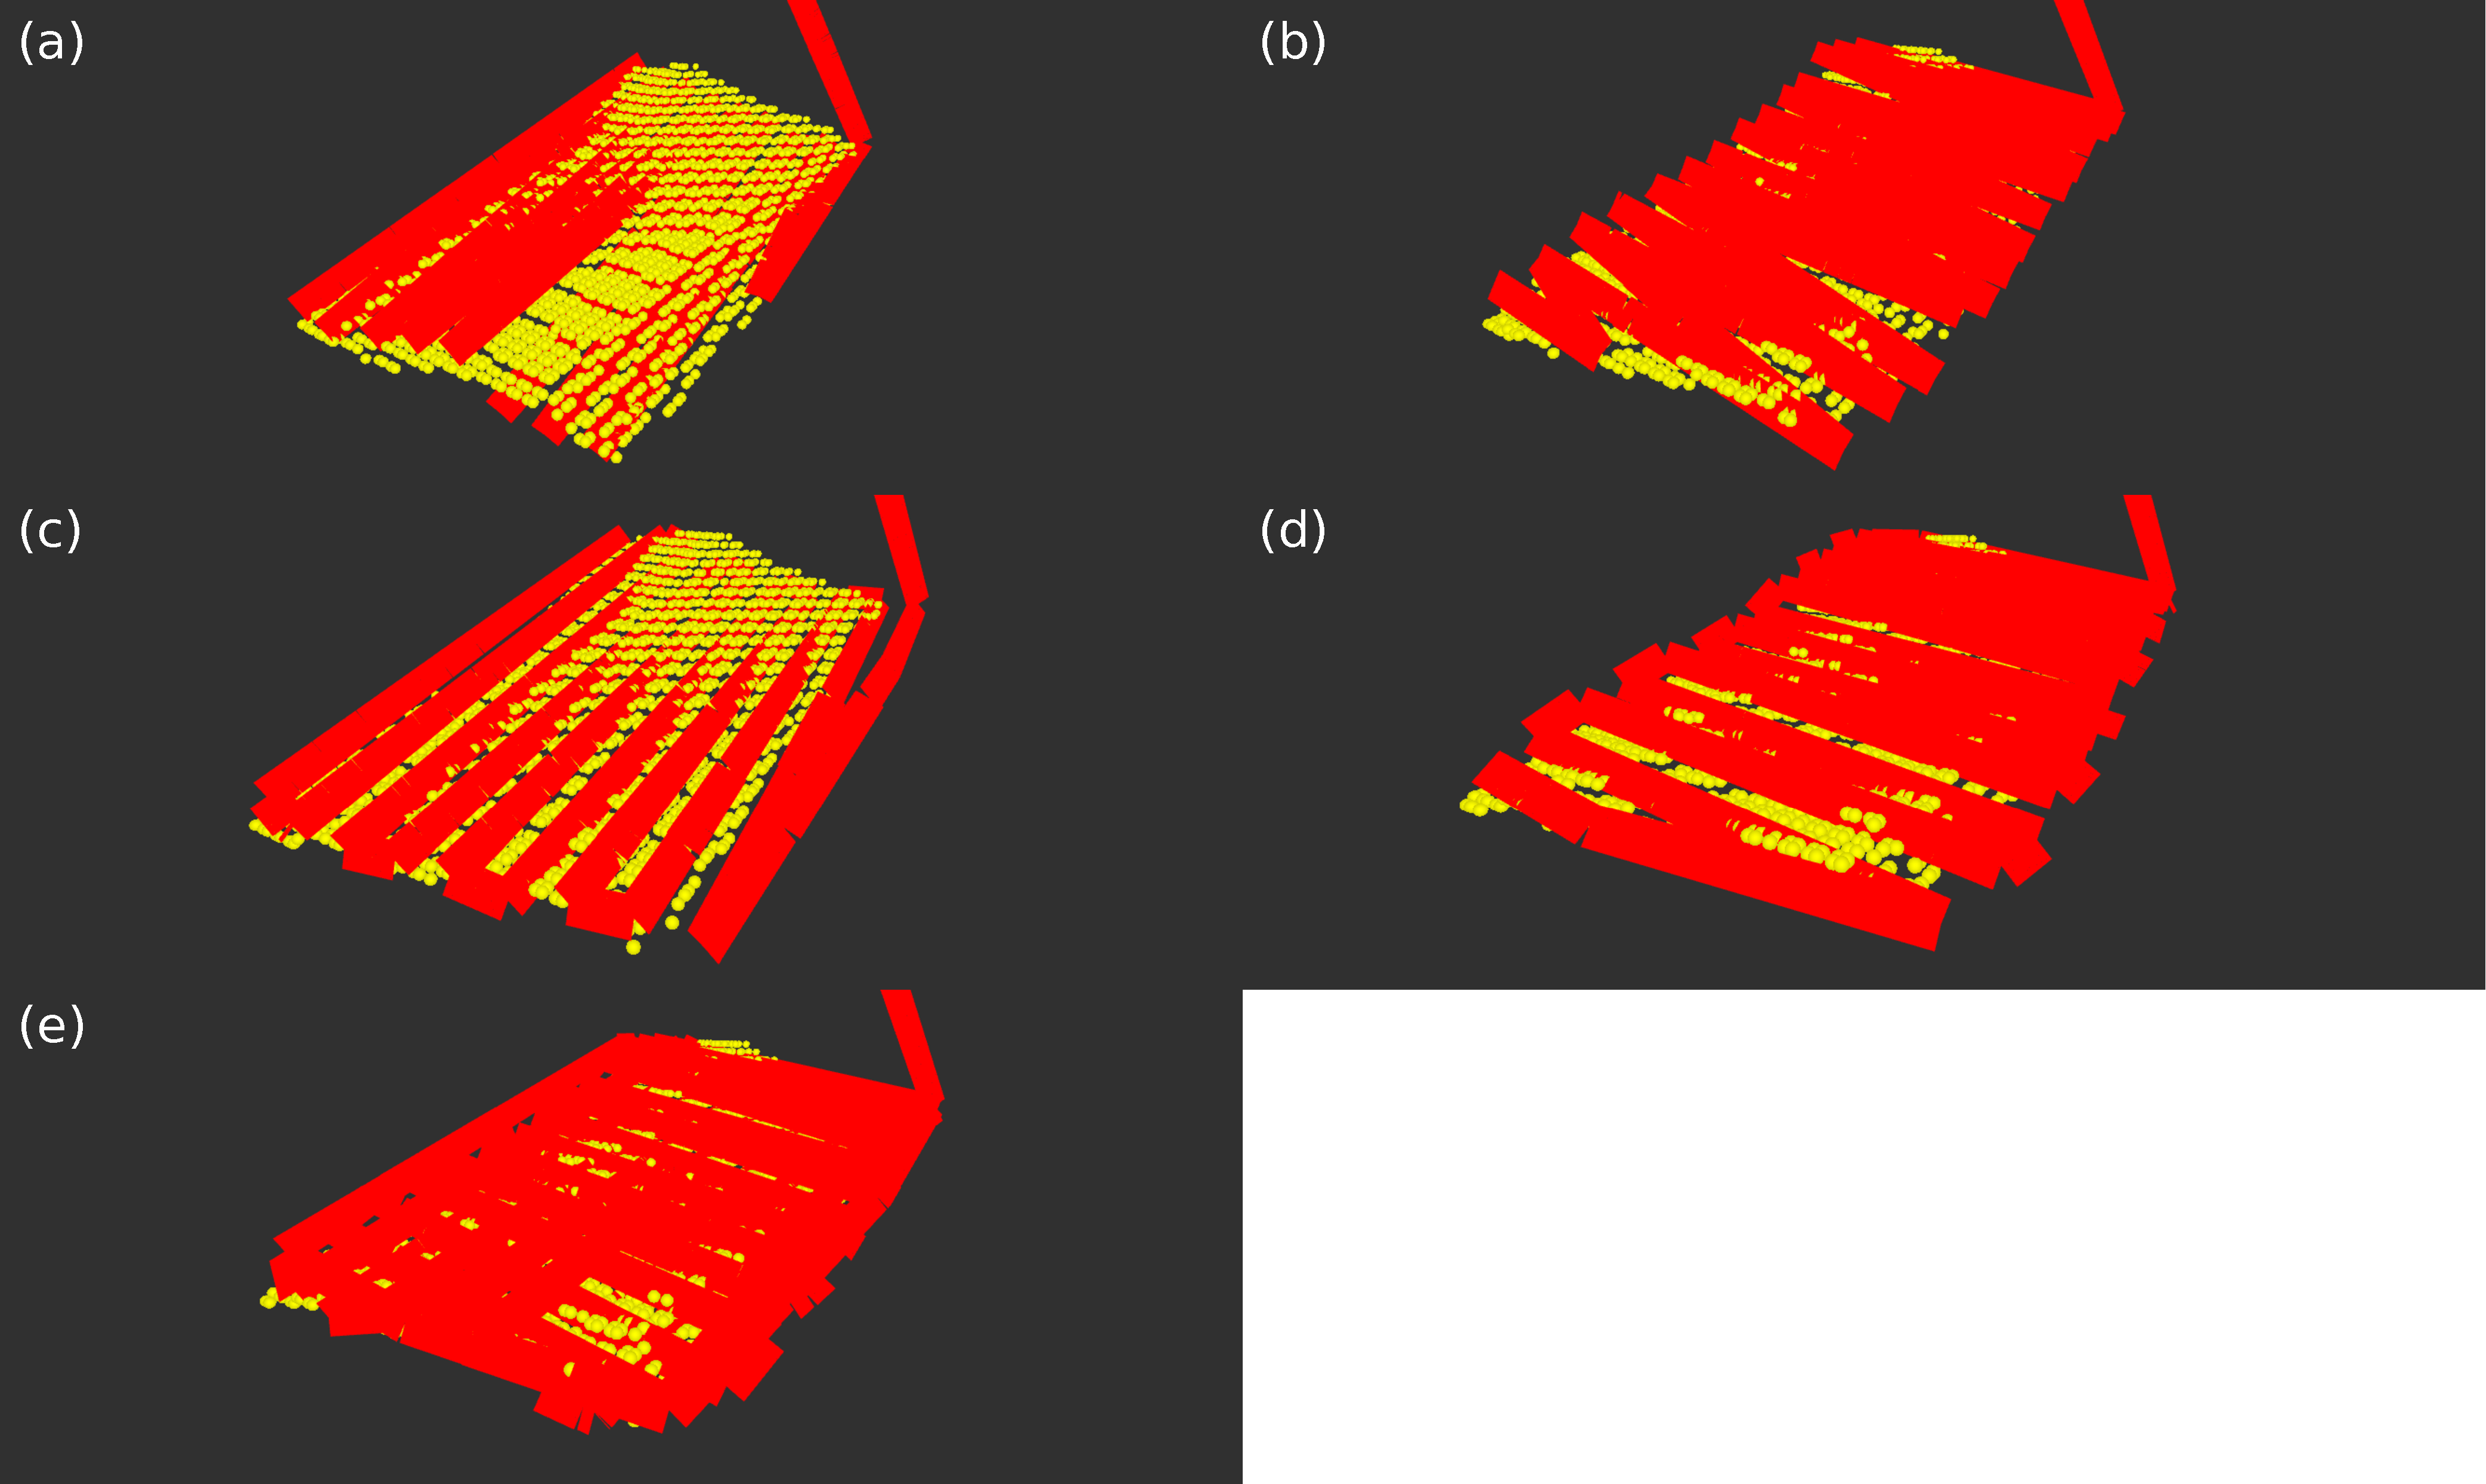
\includegraphics[width=\textwidth]{simulation_test_results_appendix_trajectory_wound_1}
	\caption[Wound 1 printing trajectory.]{Wound 1 printing trajectory. (a) ZigZag X, (b) ZigZag Y, (c) Parallel Lines X, (d) Parallel Lines Y, and (e) Grid path. All paths used $L = 5$.}
    \label{fig:simulation_test_results_toolpath_wound_1}
\end{figure}

As it can be seen on Figure \ref{fig:simulation_test_results_toolpath_wound_1}, the trajectory covers the majority of the wound. The downside is that it does not conform perfectly to the wound curvature. This problem is related to the conversion of the path from 2D image frame to 3D robot base frame, and trajectory planning.

To better analyse the quality of the trajectory execution, the trajectory tracking plots are shown for each path. Figures  \ref{fig:simulation_test_results_trajectory_wound_1_zigzag_x}, \ref{fig:simulation_test_results_trajectory_wound_1_zigzag_y}, \ref{fig:simulation_test_results_trajectory_wound_1_parallel_x}, \ref{fig:simulation_test_results_trajectory_wound_1_parallel_y}, and \ref{fig:simulation_test_results_trajectory_wound_1_grid}. 

\begin{figure}[htbp]
	\centering
	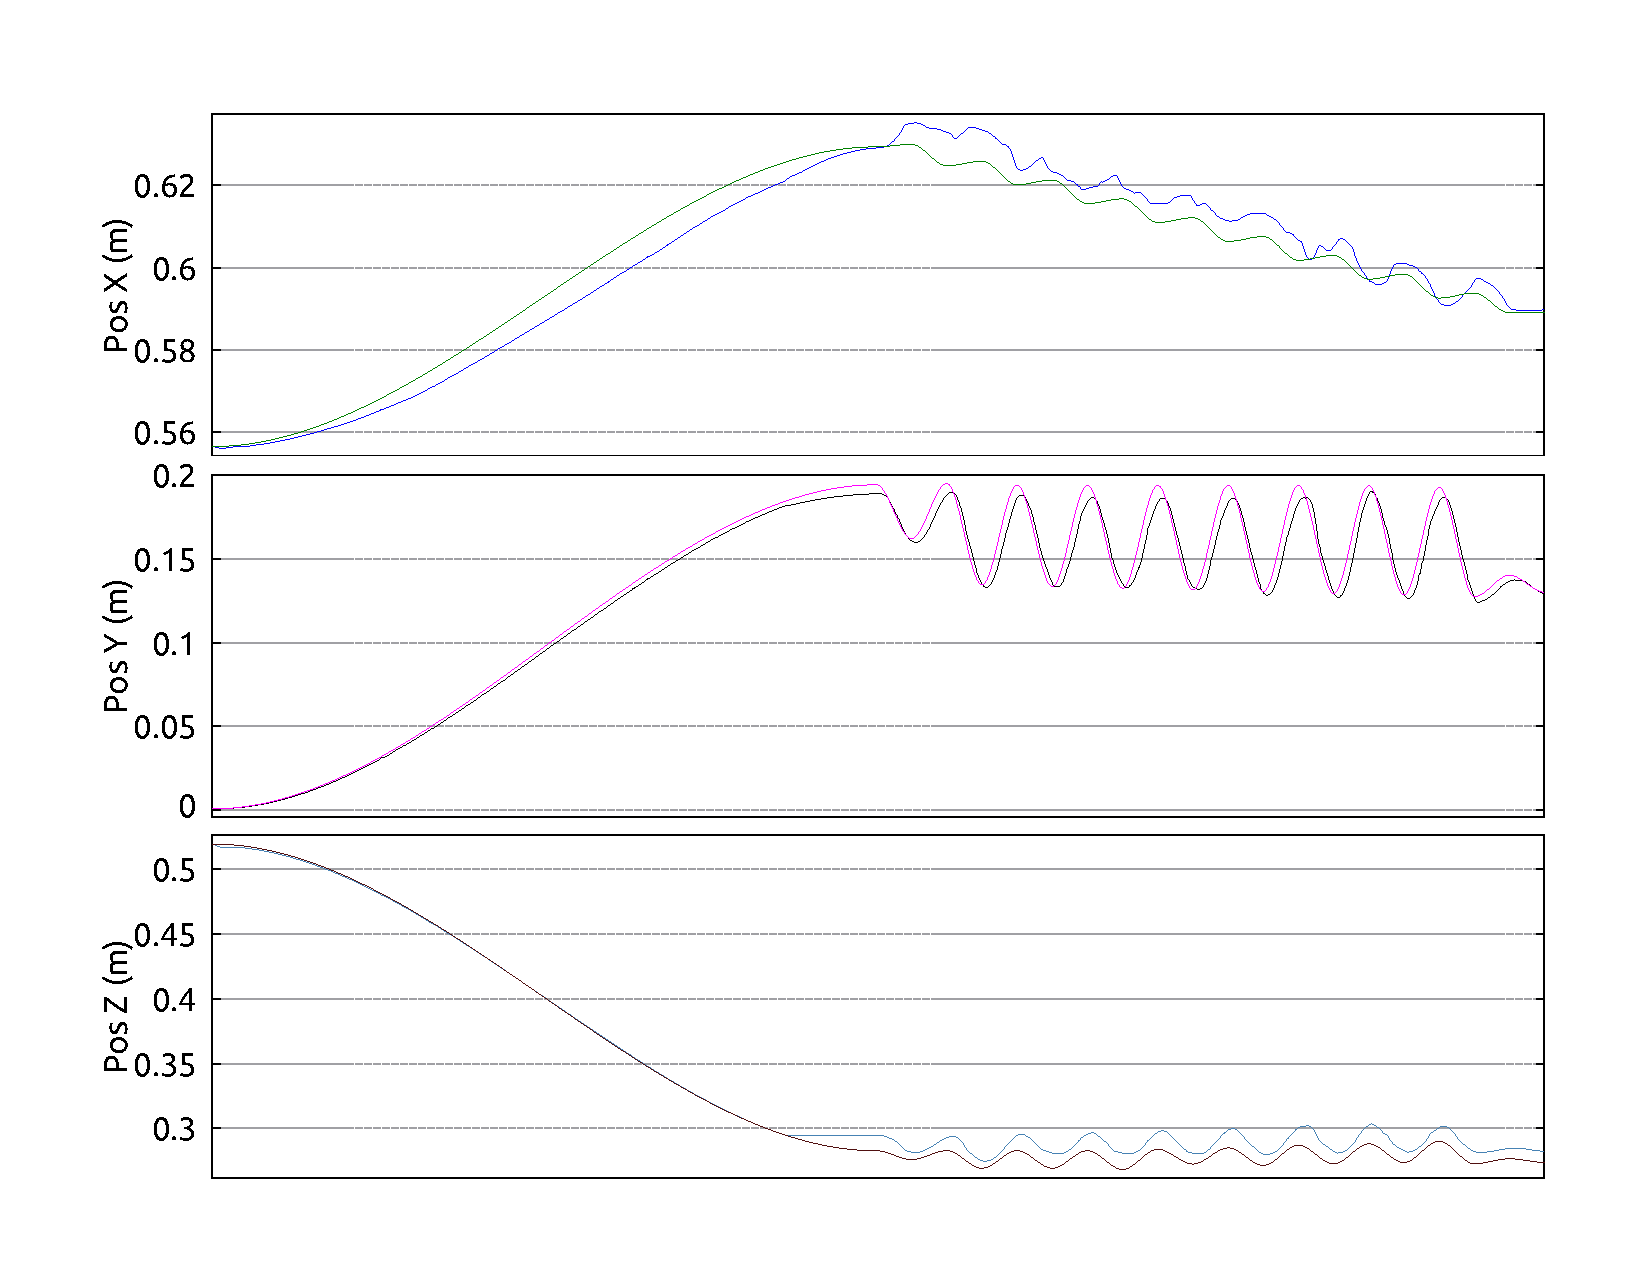
\includegraphics[width=.49\textwidth]{wound_0_zigzag_x_L5_20sec_position_track}
	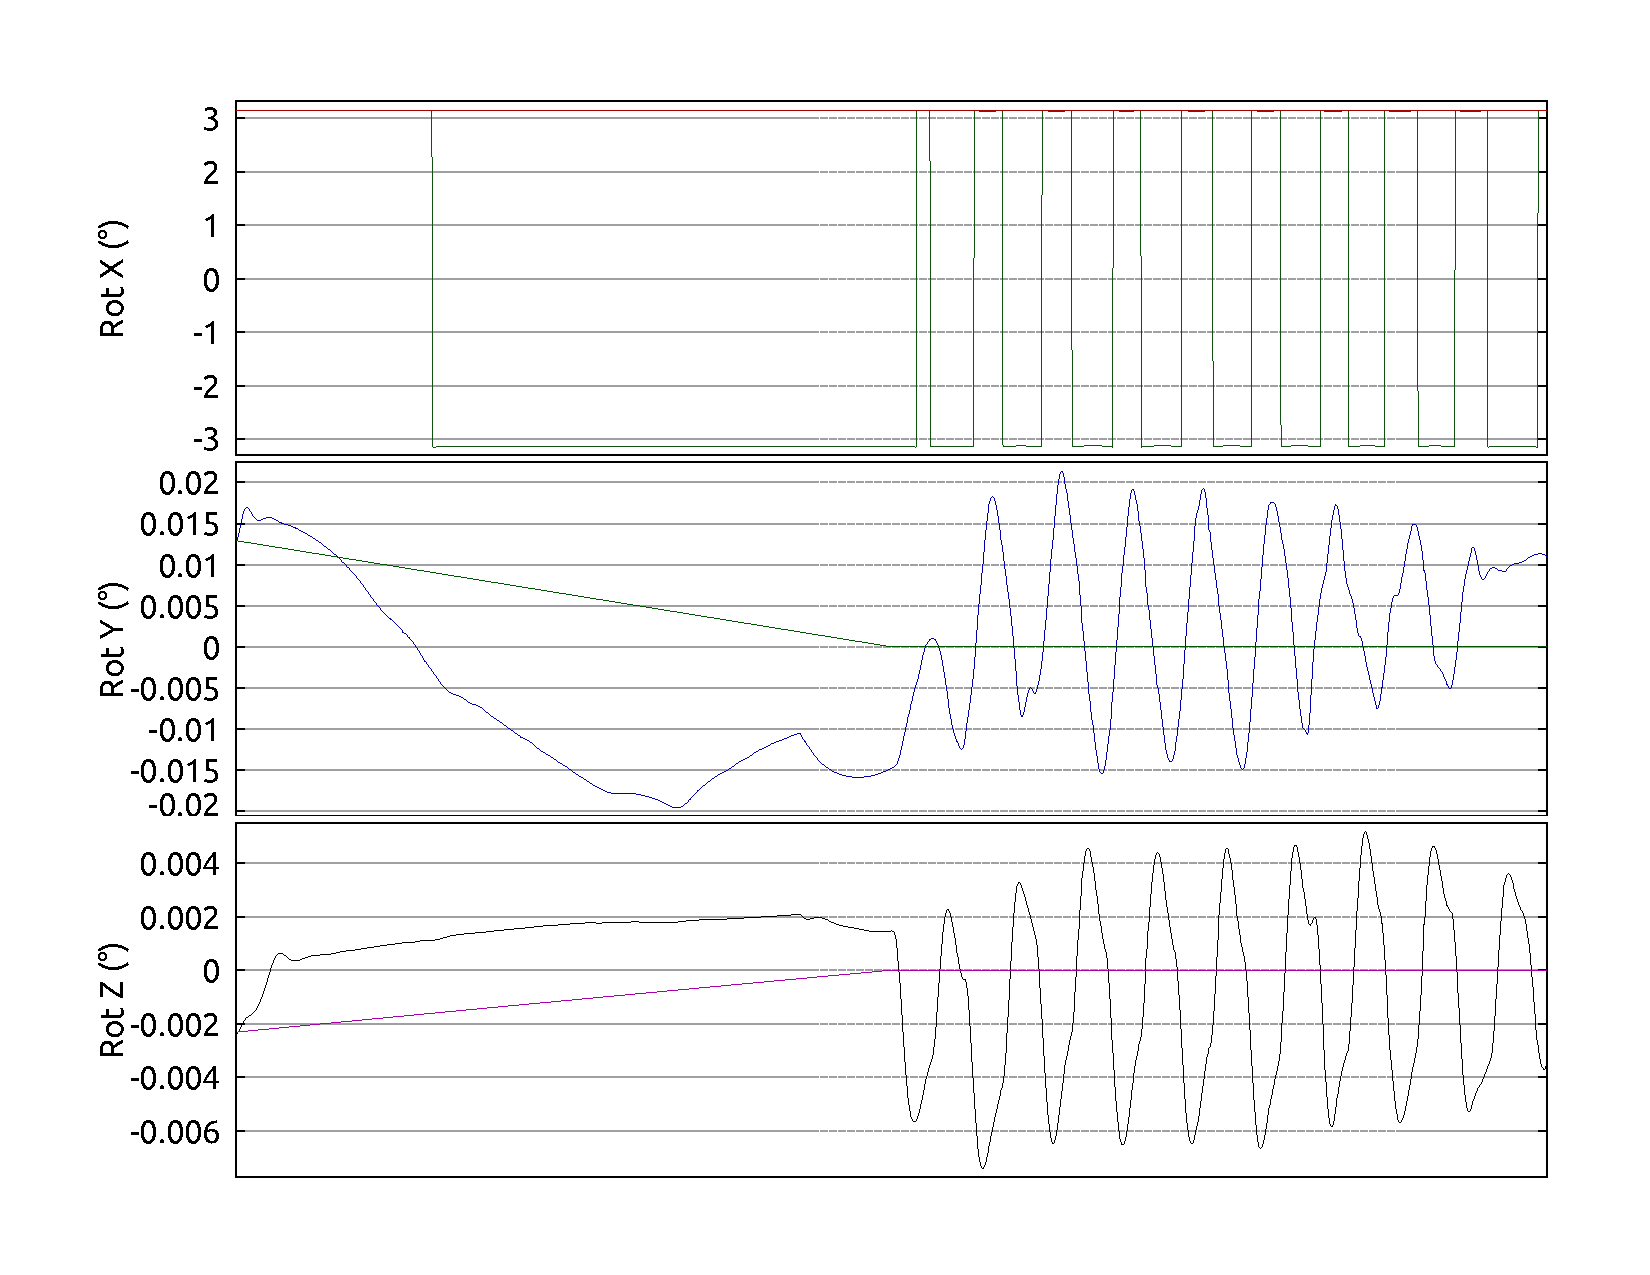
\includegraphics[width=.49\textwidth]{wound_0_zigzag_x_L5_20sec_orientation_track}
	\caption[Wound model 1 trajectory tracking plots for ZigZag X.]{Wound model 1 trajectory tracking plots for ZigZag X. (left) Desired position and current position for three axis. (right) Desired orientation and current orientation using Euler angles, for three axis.}
    \label{fig:simulation_test_results_trajectory_wound_1_zigzag_x}
\end{figure}

\begin{figure}[htbp]
	\centering
	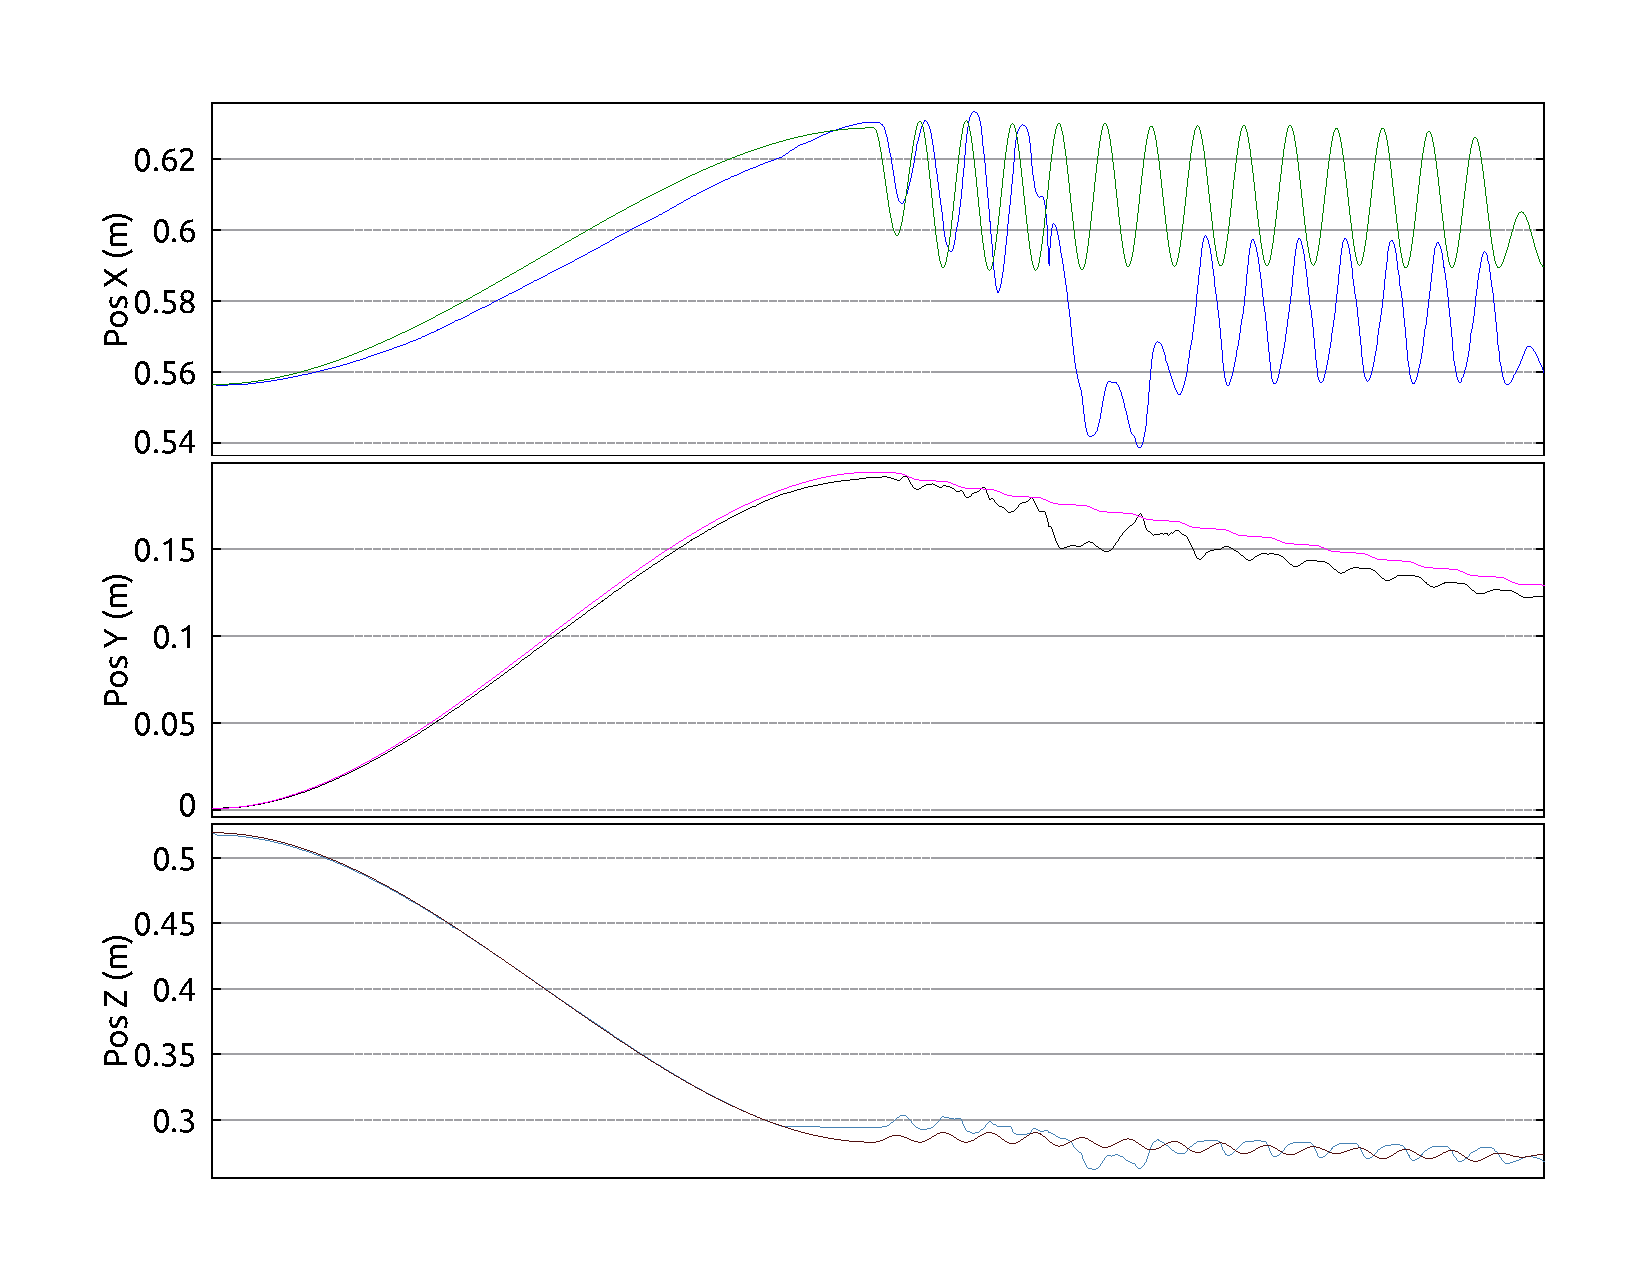
\includegraphics[width=.49\textwidth]{wound_0_zigzag_y_L5_20sec_position_track}
	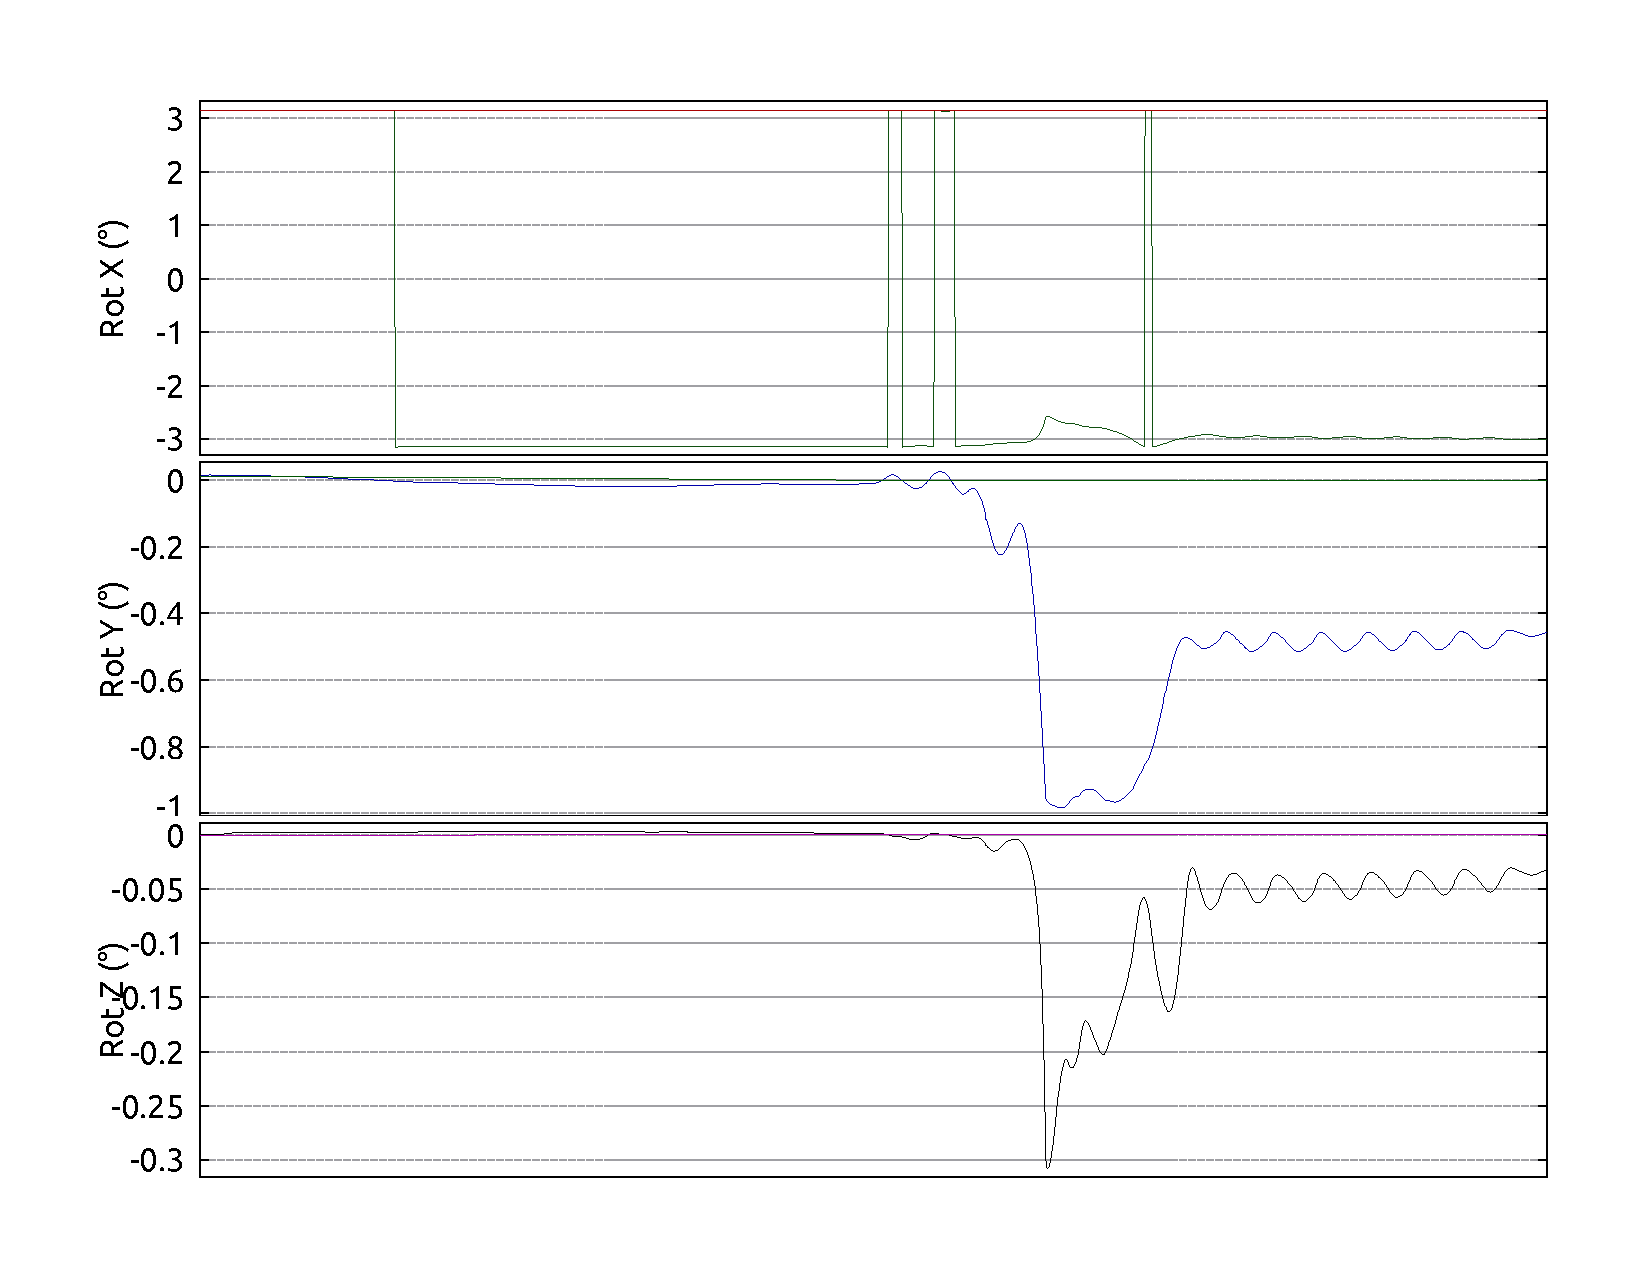
\includegraphics[width=.49\textwidth]{wound_0_zigzag_y_L5_20sec_orientation_track}
	\caption[Wound model 1 trajectory tracking plots for ZigZag Y.]{Wound model 1 trajectory tracking plots for ZigZag Y. (left) Desired position and current position for three axis. (right) Desired orientation and current orientation using Euler angles, for three axis.}
    \label{fig:simulation_test_results_trajectory_wound_1_zigzag_y}
\end{figure}

\begin{figure}[htbp]
	\centering
	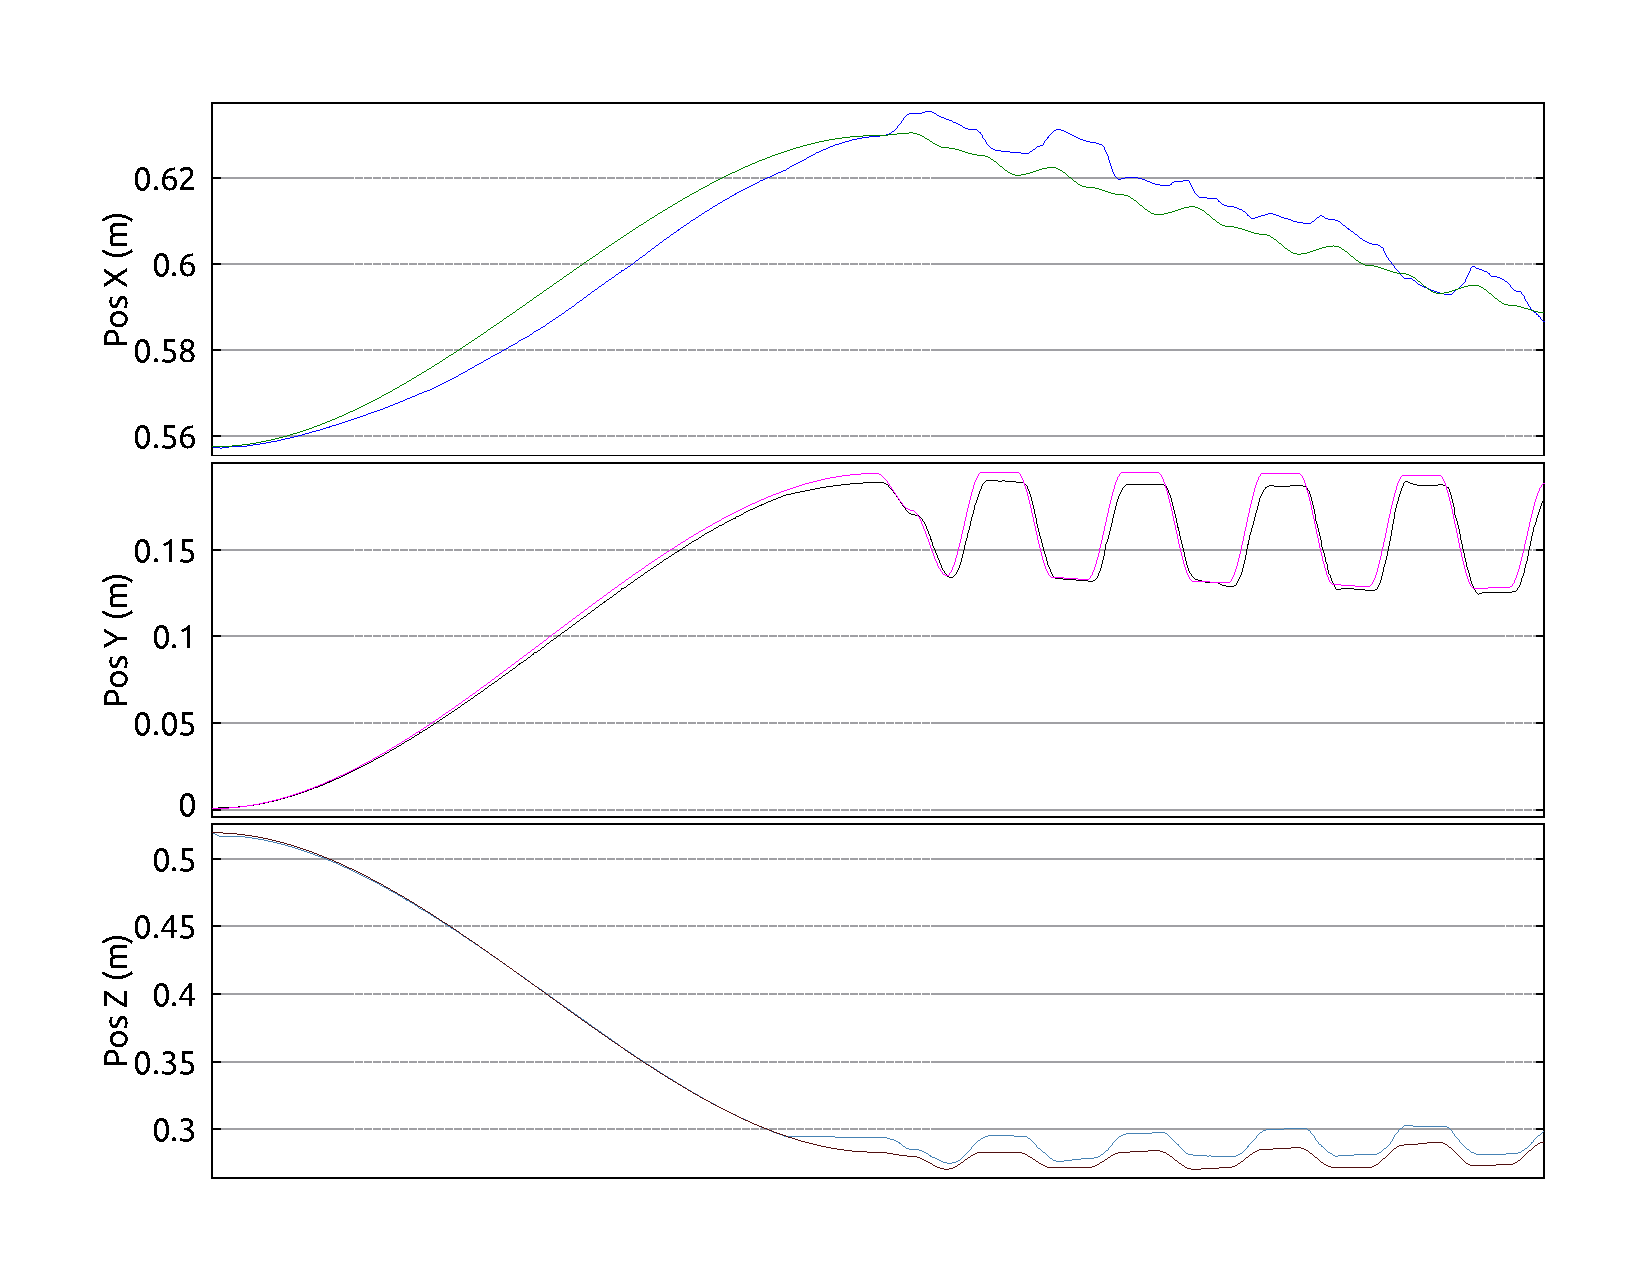
\includegraphics[width=.49\textwidth]{wound_0_parallel_x_L5_20sec_position_track}
	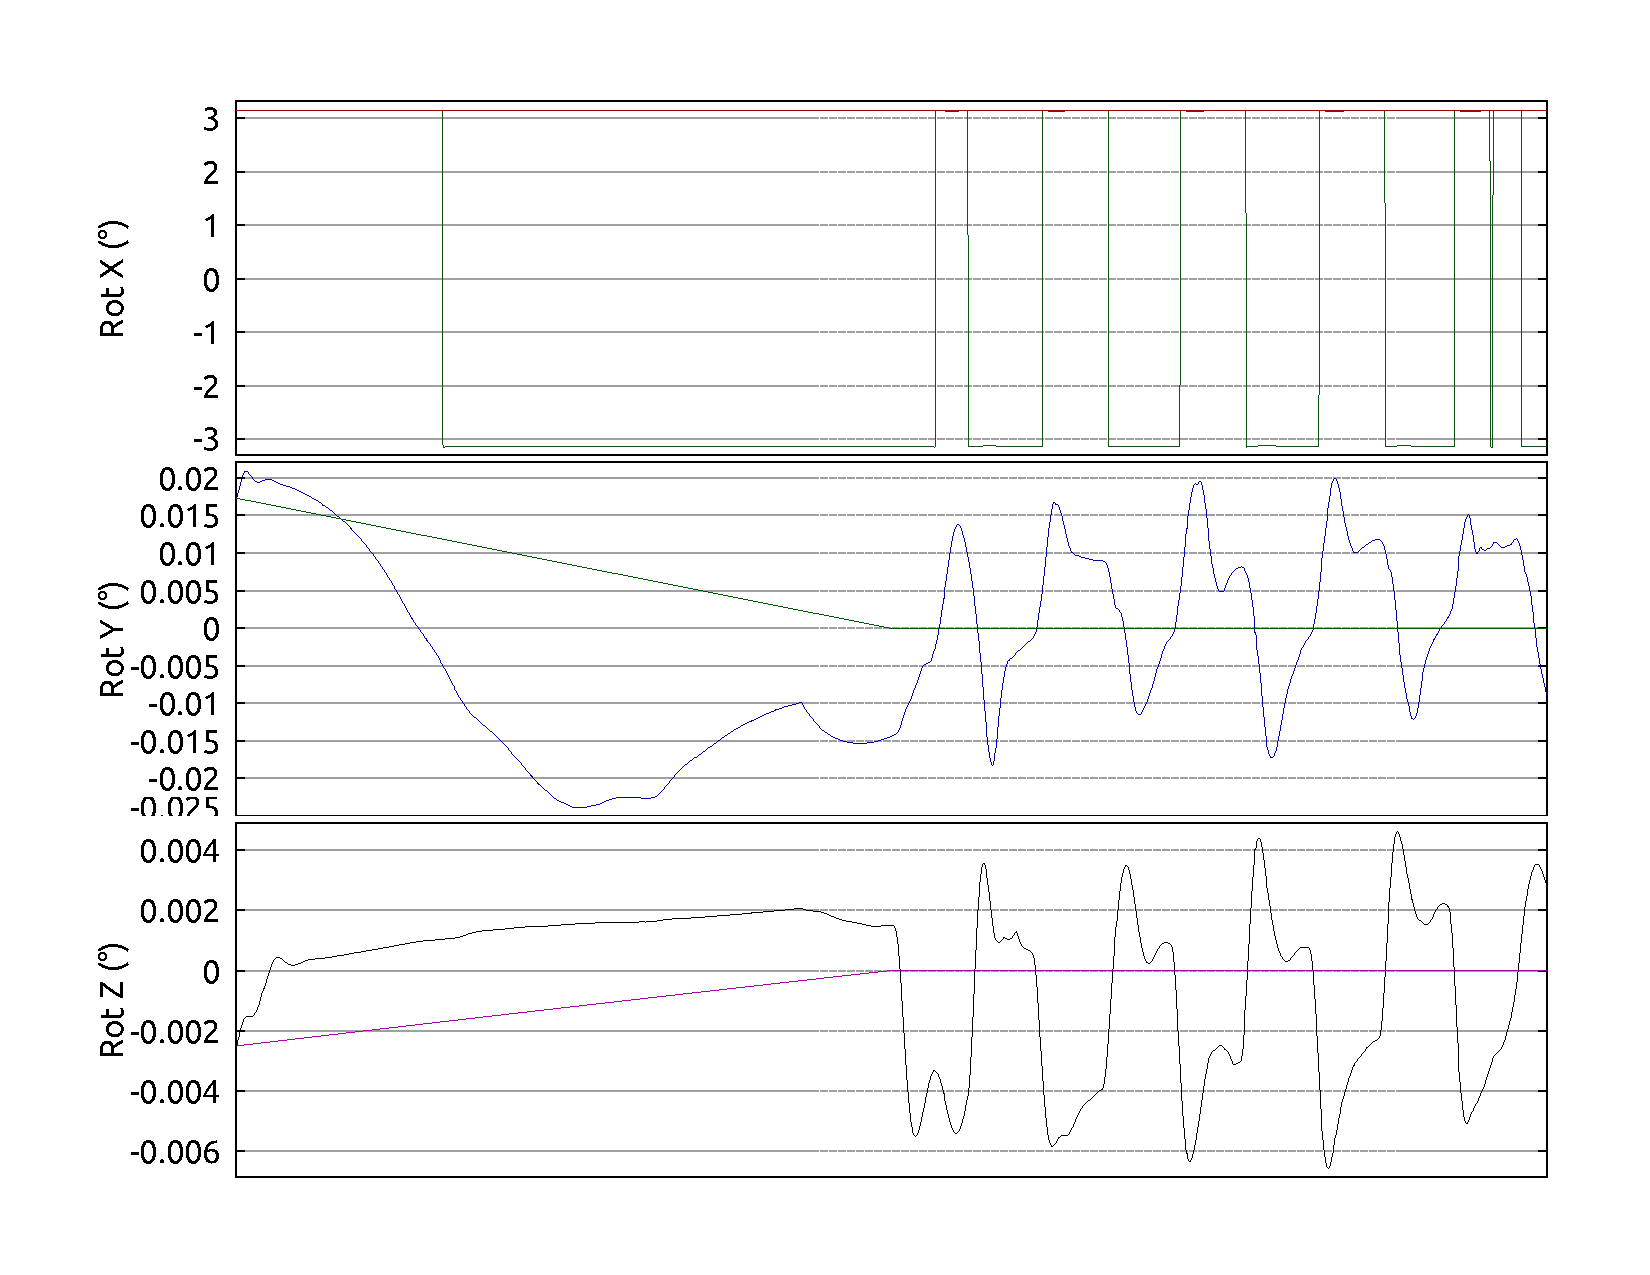
\includegraphics[width=.49\textwidth]{wound_0_parallel_x_L5_20sec_orientation_track}
	\caption[Wound model 1 trajectory tracking plots for Parallel Lines X.]{Wound model 1 trajectory tracking plots for Parallel Lines X. (left) Desired position and current position for three axis. (right) Desired orientation and current orientation using Euler angles, for three axis.}
    \label{fig:simulation_test_results_trajectory_wound_1_parallel_x}
\end{figure}

\begin{figure}[htbp]
	\centering
	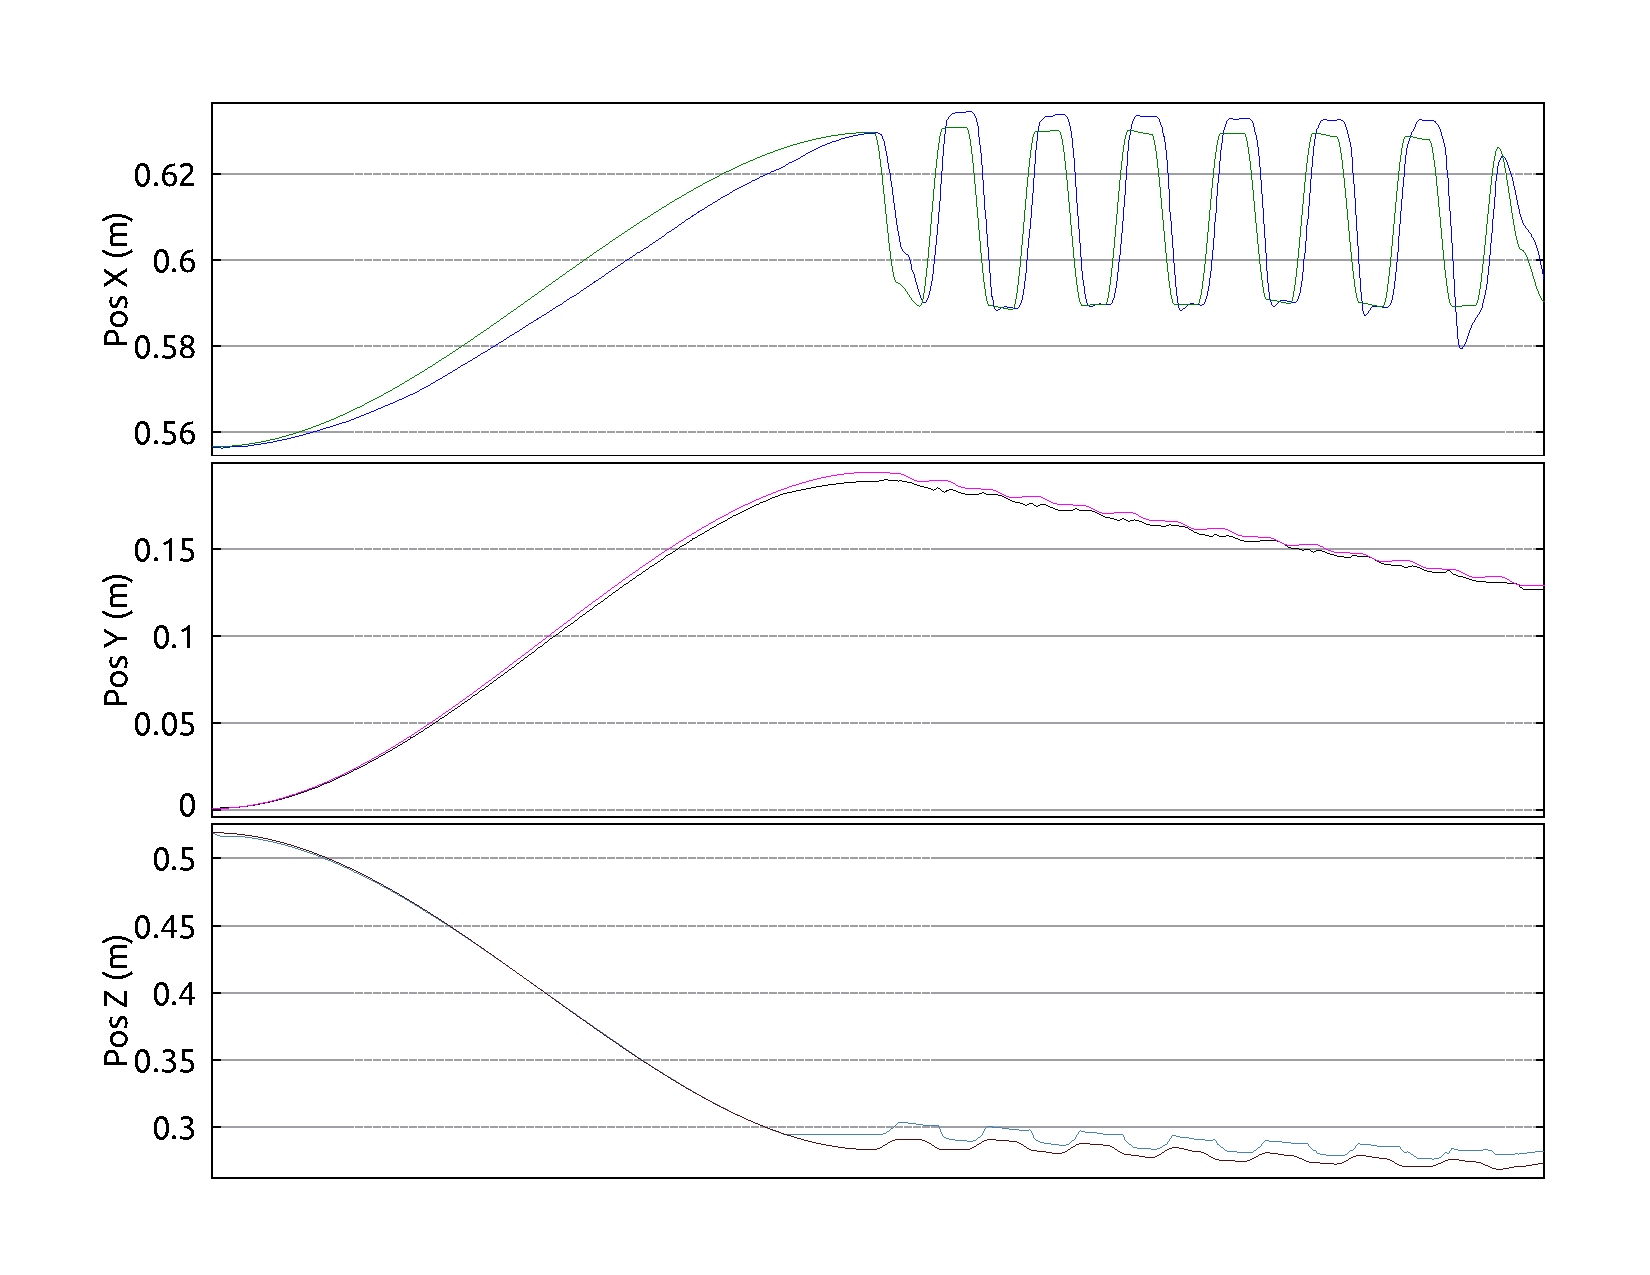
\includegraphics[width=.49\textwidth]{wound_0_parallel_y_L5_20sec_position_track}
	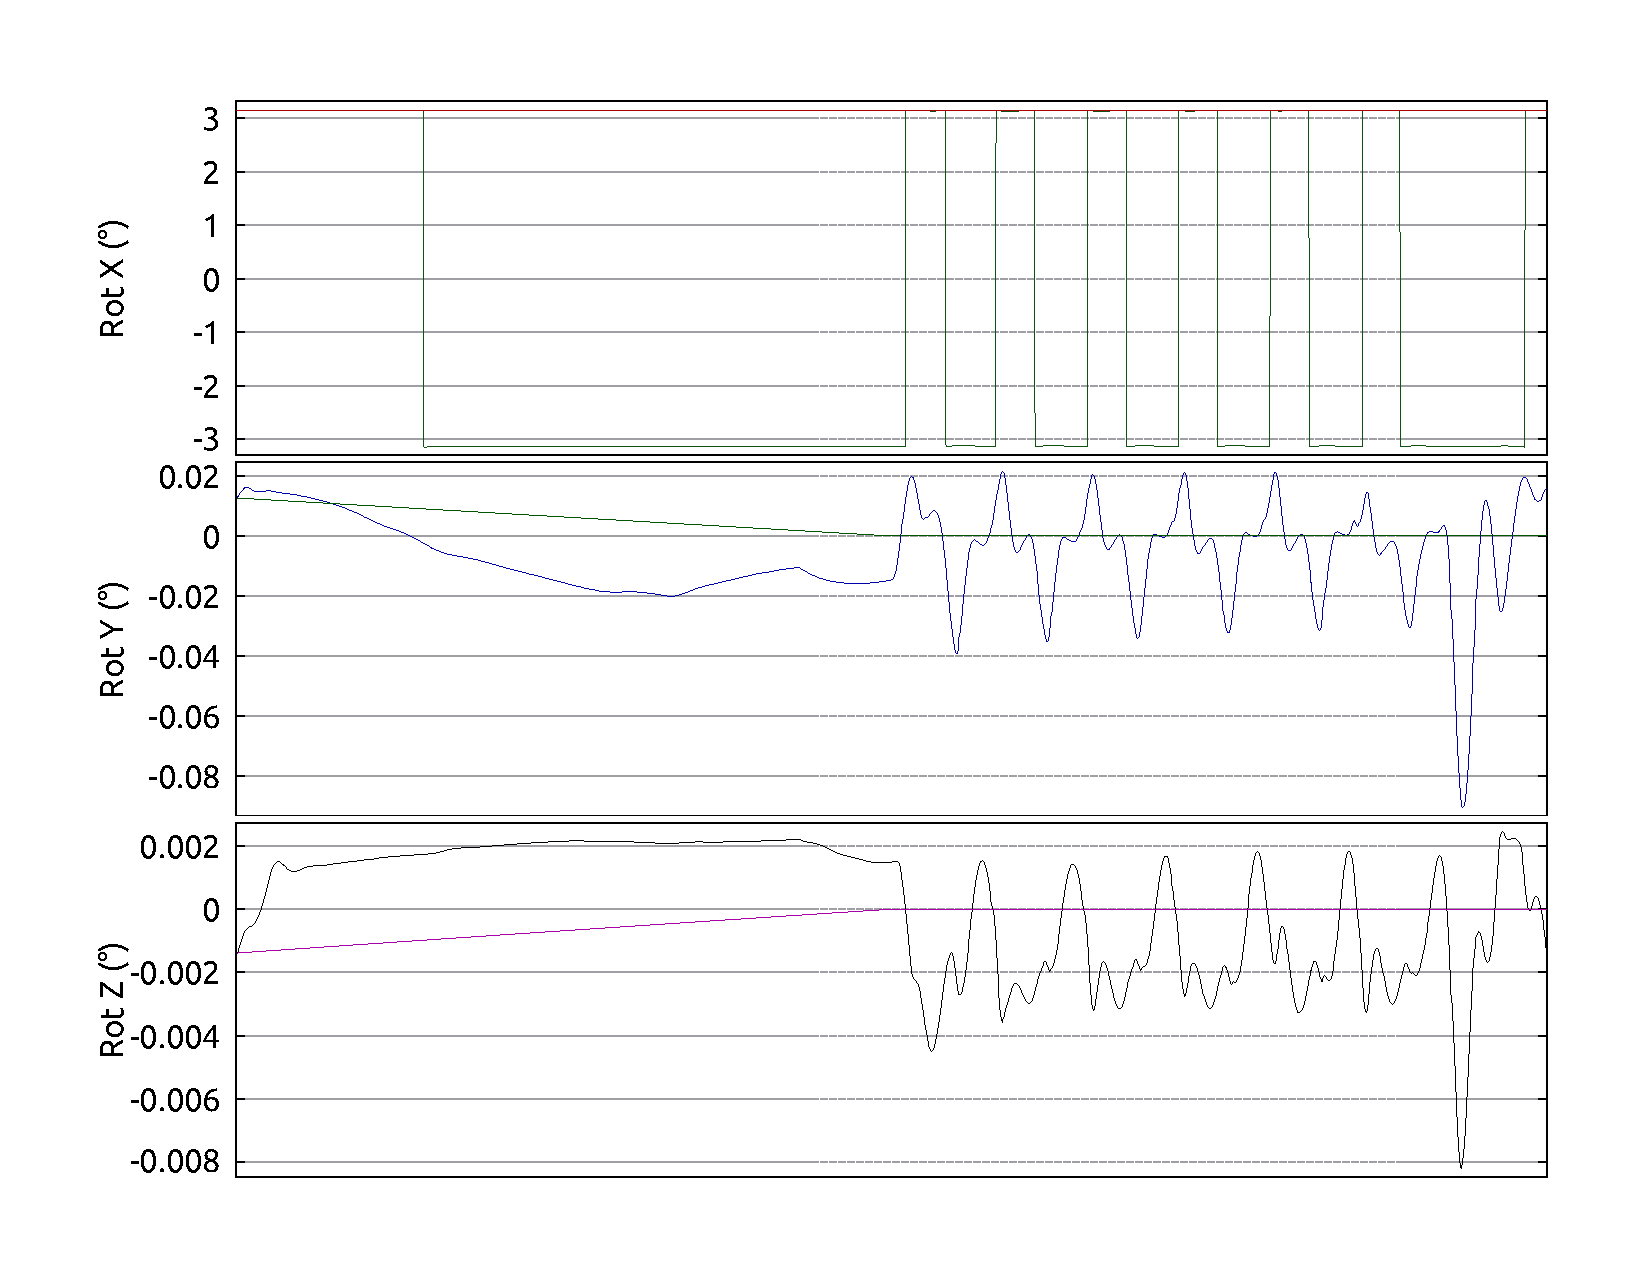
\includegraphics[width=.49\textwidth]{wound_0_parallel_y_L5_20sec_orientation_track}
	\caption[Wound model 1 trajectory tracking plots for Parallel Lines Y.]{Wound model 1 trajectory tracking plots for Parallel Lines Y. (left) Desired position and current position for three axis. (right) Desired orientation and current orientation using Euler angles, for three axis.}
    \label{fig:simulation_test_results_trajectory_wound_1_parallel_y}
\end{figure}

\begin{figure}[htbp]
	\centering
	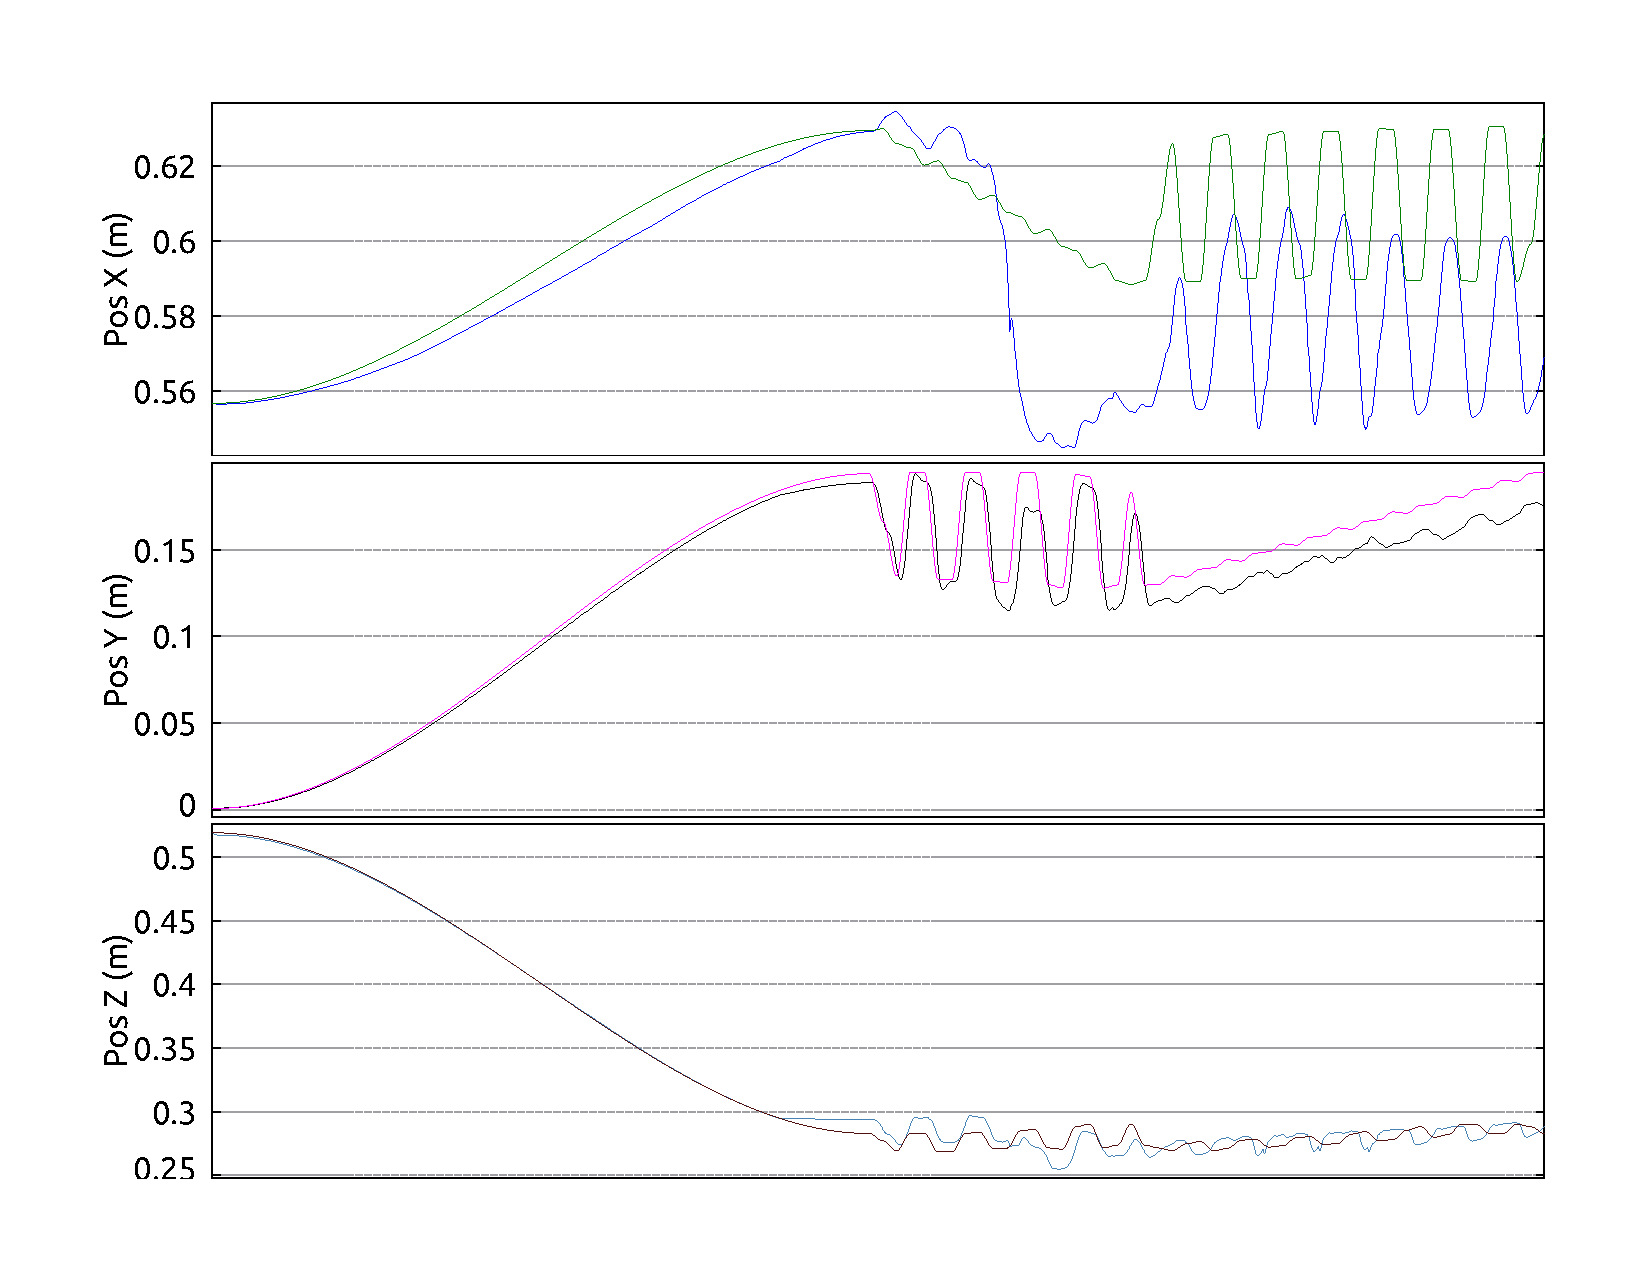
\includegraphics[width=.49\textwidth]{wound_0_grid_L5_20sec_position_track}
	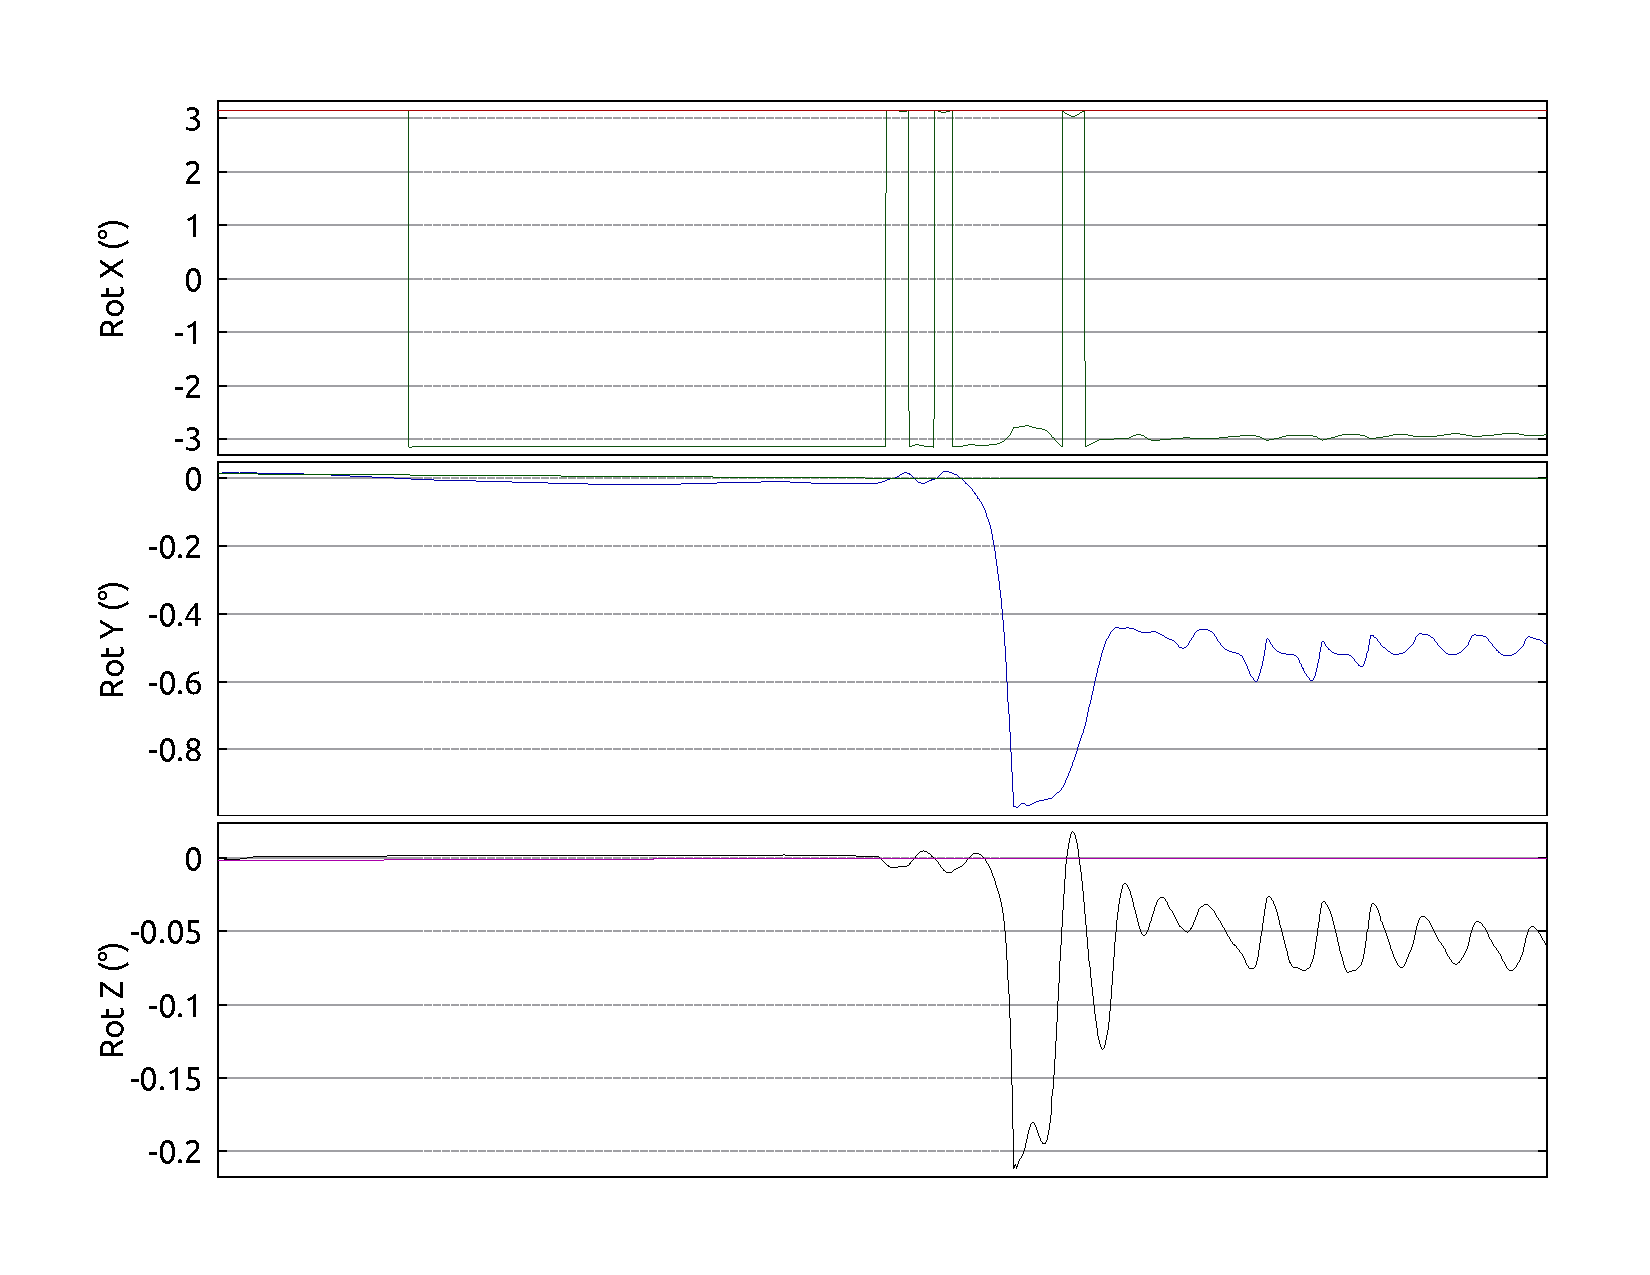
\includegraphics[width=.49\textwidth]{wound_0_grid_L5_20sec_orientation_track}
	\caption[Wound model 1 trajectory tracking plots for Grid.]{Wound model 1 trajectory tracking plots for Grid. (left) Desired position and current position for three axis. (right) Desired orientation and current orientation using Euler angles, for three axis.}
    \label{fig:simulation_test_results_trajectory_wound_1_grid}
\end{figure}

\begin{table}[htbp]
    \centering
    \caption[Trajectory tracking root mean square error for each path.]{Trajectory tracking \gls{rms} Error for each path, all the wound models. The error is calculated between the desired trajectory and the actual trajectory executed. The average time is between all the paths for each wound, considering a trajectory time of 20 seconds. The unit for position is meters, degrees for the orientation and seconds for time.}
\begin{adjustbox}{width=1.2\textwidth,center=\textwidth}
    \begin{tabular}{c|c|c|c|c|c|c|c|c}
        \toprule
         \multicolumn{2}{c|}{\textbf{Path}} & \textbf{Px} & \textbf{Py} & \textbf{Pz} & \textbf{Ox} & \textbf{Oy} & \textbf{Oz} & \textbf{Avg. Time} \\
         \midrule
         \multirow{5}{*}{\textbf{Wound 1}} & ZigZag X & 0.00353 & 0.00454 & 0.00735 & 4.09771 & 0.01106 & 0.00279 & \multirow{5}{*}{\textbf{21.042}}\\
         & ZigZag Y & 0.02652 & 0.00653 & 0.00647 & 5.28248 & 0.37018 & 0.04983 & \\
         & Parallel Lines X & 0.00444 & 0.00436 & 0.00717 & 4.68632 & 0.01469 & 0.00271 & \\
         & Parallel Lines Y & 0.00428 & 0.00285 & 0.00751 & 5.11224 & 0.01106 & 0.00167 & \\
         & Grid & 0.02204 & 0.01262 & 0.00611 & 4.67674 & 0.34219 & 0.04686 & \\
         \midrule
         \multirow{5}{*}{\textbf{Wound 2}} & ZigZag X & 0.0166 & 0.01093 & 0.00784 & 4.39807 & 0.30494 & 0.11912 & \multirow{5}{*}{\textbf{22.008}}\\
         & ZigZag Y & 0.02694 & 0.0031 & 0.00892 & 5.06093 & 0.32344 & 0.04982 & \\
         & Parallel Lines X & 0.01591 & 0.00707 & 0.00659 & 4.26746 & 0.24282 & 0.01557 &\\
         & Parallel Lines Y & 0.02422 & 0.00456 & 0.01175 & 4.81934 & 0.26827 & 0.05175 & \\
         & Grid & 0.0509 & 0.01472 & 0.0141 & 4.30018 & 0.4719 & 0.22604 & \\
         \midrule
         \multirow{5}{*}{\textbf{Wound 3}} & ZigZag X & 0.01832 & 0.01612 & 0.00608 & 4.34085 & 0.28366 & 0.05087 & \multirow{5}{*}{\textbf{21.986}}\\
         & ZigZag Y & 0.02858 & 0.00731 & 0.00327 & 5.29049 & 0.44922 & 0.17453 & \\
         & Parallel Lines X & 0.01445 & 0.01426 & 0.00566 & 4.11836 & 0.33327 & 0.11517 & \\
         & Parallel Lines Y & 0.02998 & 0.00844 & 0.00406 & 4.62167 & 0.51299 & 0.26446 &\\
         & Grid & 0.01849 & 0.0228 & 0.00927 & 4.37902 & 0.50123 & 0.16542 &\\
         \midrule
         \multirow{5}{*}{\textbf{Wound 4}} & ZigZag X & 0.00333 & 0.01005 & 0.00481 & 4.70069 & 0.00784 & 0.00368 & \multirow{5}{*}{\textbf{23.119}}\\
         & ZigZag Y & 0.02172 & 0.00262 & 0.00606 & 3.19297 & 0.2488 & 0.0172 & \\
         & Parallel Lines X & 0.00384 & 0.00856 & 0.00453 & 4.23706 & 0.01472 & 0.00356 & \\
         & Parallel Lines Y & 0.01272 & 0.00269 & 0.00798 & 3.63359 & 0.15849 & 0.03952 & \\
         & Grid & 0.0242 & 0.02556 & 0.00747 & 4.46427 & 0.29853 & 0.05155 &\\
         \midrule
         \multirow{5}{*}{\textbf{Wound 5}} & ZigZag X & 0.01954 & 0.00584 & 0.00484 & 4.71366 & 0.30595 & 0.03255 & \multirow{5}{*}{\textbf{20.273}}\\
         & ZigZag Y & 0.02855 & 0.00333 & 0.0069 & 4.71507 & 0.37293 & 0.03612 & \\
         & Parallel Lines X & 0.00378 & 0.00419 & 0.00628 & 4.46086 & 0.01175 & 0.00266 &\\
         & Parallel Lines Y & 0.03223 & 0.00409 & 0.01007 & 3.27704 & 0.55023 & 0.09593 & \\
         & Grid & 0.01624 & 0.00817 & 0.00556 & 4.62273 & 0.57879 & 0.23749 & \\
         \bottomrule
    \end{tabular}
    \label{tab:cartesian_impedance_tracking_rmse}
\end{adjustbox}
\end{table}

% subsection simulated_system_results_bioprinting_directly_wound

% section system_validation_simulation_results

% ==========================
% = Discussion =
% ==========================

\clearpage

\section{Discussion}
\label{sec:system_validation_discussion}

From all the results obtained it is clear the system depends heavily on the vision system. Things like camera calibration will have a direct impact on the results.

One example of this dependence is the fact the all the data obtained for the wounds, with the camera, depends completely on the camera orientation. If the camera detects the wound but is not at the best angle, the detection may be partial which means the whole wound filling procedure will fail. On the tests conducted, the camera was always positioned in a way that the whole wound area was visible by it.

With this in mind, Figure \ref{fig:system_validation_simulation_results_wound_detection_segmentation} shows that the segmentation algorithm used was capable of segmenting the wounds correctly. Although the results are not available, some tests were conducted with a real camera that showed that the algorithm had limitations. The lighting has a big effect on the color perceived and the threshold can fail. Even the Otsu method was tried but still had problems. For a real application, the algorithm must not depend much on the lighting conditions. Besides, it must also be an algorithm that works on real wound images.\\

Obtaining spatial data is also essential for validating the concept. The position data had some validation problems. The conversion between the camera frame to the robot base frame produced a reduced and dislocated model of the wound, seen by the point cloud created (Fig. \ref{fig:simulation_test_results_camera_spatial_data_wound_position_test_results}). This has to do with camera calibration problems or the lack of camera calibration and some flaw on the conversion algorithm. However, the limitations of the present work do not mean it cannot be done. As seen on the literature review, this flaw is surpassed by other works and does not consist on a scientific limitation. Nonetheless, although the position and scale after conversion is wrong, the wound shape is still conserved by the point cloud (Fig. \ref{fig:simulation_test_results_camera_spatial_data_wound_pcloud_mesh_resume}). On table \ref{tab:wound_position_results} it is possible to see that the absolute errors are on the order of centimeters, with the maximum being around 3 cm on the y direction.

The values obtained for wound area and perimeter are also wrong. It is understandable since the wound position data has errors too. To try to validate the algorithm independently of the wound position errors, the perimeter and area were also calculated with the detected points data, and compared with the algorithm values. On tables \ref{tab:wound_area_results} and \ref{tab:wound_perimeter_results}, the last column shows these errors. The errors are non-zero but are less than the errors between the algorithm and the expected values. Another related detail to consider is that the area and perimeter calculation may work well on planar wounds but it will fail on non-planar wounds. It depends heavily on the camera orientation. The mesh is probably the best tool to measure the area and perimeter correctly. This measurement was not done.

The spatial data results completely invalidate the use of the system. If the system cannot calculate the precise position of the wound, it cannot bioprint directly on it.\\

Even with bad spatial data, the path planning still work fairly well on the wound shape detected. The path planning produced good results on the x-y plane. On the z-axis, the path did not respected the wound shape. As seen in Figure \ref{fig:simulation_test_results_toolpath_wound_1}, some paths were not executed completely on top of the wound but went on the bottom. This means it would go inside the wound which is not desirable. Even considering that the printing will be done at least 0.5 to 1 cm above the wound, not following the wound shape can present problems. This limitation was related to the way the lines were calculated. When building the path, only the extreme points were match to the z-axis. This means that an elevation on the middle of the wound would not be considered and the line would pass right through. To fix this, the lines need to be decomposed into more points that are matched against the point cloud for z-axis.\\

The wound filling trajectory execution was effectively executed for all paths and wound models, with the impedance gains used. However, the tracking was far from perfect. The position tracking was better than orientation. It had \gls{rms} errors on the order of centimeters, sometimes millimeters. It is not satisfactory for the desired goal. The orientation errors were higher, specially for rotations about the x-axis, were errors of 5 degrees were obtained. The impedance gains need some fine tuning to improve the trajectory execution precision.

If we look at table \ref{tab:cartesian_impedance_tracking_rmse}, we can see that the trajectory times were not fully respected. The goal was 20 seconds for each path on each wound, but the average time for each wound is at least one second above it. It does not mean that the planning failed, but that the complete execution uses more resources that can affect the execution time. \\

Overall, despite some flaws, the system implemented demonstrated that it is possible to execute a wound filling bioprinting trajectory using a robotic arm paired with a vision system, with some degree of autonomy. If each layer is corrected and optimised, the system will be able to do its job with enough precision to be effective.

% section system_validation_discussion